\documentclass[runningheads]{llncs}
% RECOMB format: US Letter, 1-inch margins, 10pt.
\usepackage[letterpaper,margin=1in]{geometry}
\usepackage[T1]{fontenc}
\usepackage{lmodern}
\usepackage{amsmath,amssymb}
\usepackage{graphicx}
\usepackage{booktabs}
\usepackage{longtable}
\usepackage{xcolor}
\usepackage[hidelinks]{hyperref}
\usepackage{microtype}
\usepackage{placeins}

\newcommand{\Cov}{\mathrm{Cov}}
\newcommand{\Qt}{\mathrm{Quant}}
\newcommand{\1}{\mathbf{1}}
\newcommand{\E}{\mathbb{E}}
\renewcommand{\P}{\mathbb{P}}
\newcommand{\dtv}{d_{\mathrm{TV}}}
% Generated by scripts/make_tables.py from results/; do not edit.
\newcommand{\nProteins}{2,525}
\newcommand{\nVariants}{62,727}
\newcommand{\fracPath}{51.0\%}
\newcommand{\medVar}{12}
\newcommand{\maxVar}{741}
\newcommand{\minVar}{2}
\newcommand{\nUniprot}{2,489}
\newcommand{\nFam}{2,081}
\newcommand{\nFamSingleton}{1,805}
\newcommand{\nFamGeTen}{1,309}
\newcommand{\nFamOrphan}{1,276}
\newcommand{\maxFamSize}{10}
\newcommand{\nFamFifty}{2,275}
\newcommand{\nFamHC}{1,939}
\newcommand{\signMaxDiff}{0.000}
\newcommand{\pubAucRange}{0.892--0.920}
\newcommand{\baseAucRange}{0.873--0.929}
\newcommand{\nTrainFam}{832}
\newcommand{\nCalFam}{624}
\newcommand{\nTestFam}{625}
\newcommand{\nCalConfFam}{416}
\newcommand{\sTwoCalMaxId}{0.221}
\newcommand{\sTwoTestMaxId}{0.105}
\newcommand{\sTwoCalNeff}{6.93}
\newcommand{\sTwoTestNeff}{5.88}
\newcommand{\sTwoEssFrac}{0.51}
\newcommand{\sTwoBtwoEssFrac}{0.25}
\newcommand{\sTwoBtwoClipped}{2.0\%}
\newcommand{\sThreeCalMaxId}{0.236}
\newcommand{\sThreeTestMaxId}{0.048}
\newcommand{\sOneBtwoPath}{0.749--0.790}
\newcommand{\sOneBtwoPathTrancept}{0.928}
\newcommand{\sOneBtwoPathVar}{0.893--0.905}
\newcommand{\sOneBoneCovFam}{0.880--0.885}
\newcommand{\sOneBoneCovVar}{0.894--0.901}
\newcommand{\sOneHcpCovFam}{0.900--0.901}
\newcommand{\sOneHcpccPath}{0.898--0.904}
\newcommand{\sOneHcpccBenign}{0.898--0.903}
\newcommand{\sOnePwPath}{0.895--0.904}
\newcommand{\sTwoBoneHcpPath}{0.838--0.908}
\newcommand{\sTwoBoneHcpBenign}{0.875--0.927}
\newcommand{\sTwoBoneGwcpPath}{0.888--0.899}
\newcommand{\sTwoBoneGwcpBenign}{0.894--0.909}
\newcommand{\sTwoBonePwPath}{0.895--0.910}
\newcommand{\sTwoBonePwBenign}{0.898--0.909}
\newcommand{\sTwoBoneBtwoPath}{0.655--0.920}
\newcommand{\sTwoBoneBtwoBenign}{0.839--0.929}
\newcommand{\sTwoBonePwPathEsm}{0.910}
\newcommand{\sTwoBoneHcpPathEsm}{0.838}
\newcommand{\sTwoBoneBtwoPathNT}{0.655--0.795}
\newcommand{\sTwoBonePwSize}{1.290--1.428}
\newcommand{\sTwoBoneHcpSize}{1.260--1.329}
\newcommand{\sTwoBoneGwcpSize}{1.269--1.397}
\newcommand{\sTwoBoneDiffGwcp}{+0.002 to +0.012}
\newcommand{\sTwoBoneDiffGwcpNpos}{5}
\newcommand{\sTwoBoneDiffHcpEsm}{+0.072 [+0.067, +0.078]}
\newcommand{\sTwoBtwoHcpPath}{0.798--0.920}
\newcommand{\sTwoBtwoHcpBenign}{0.853--0.939}
\newcommand{\sTwoBtwoGwcpPath}{0.877--0.895}
\newcommand{\sTwoBtwoGwcpBenign}{0.873--0.906}
\newcommand{\sTwoBtwoPwPath}{0.896--0.910}
\newcommand{\sTwoBtwoPwBenign}{0.892--0.916}
\newcommand{\sTwoBtwoBtwoPath}{0.619--0.921}
\newcommand{\sTwoBtwoBtwoBenign}{0.839--0.941}
\newcommand{\sTwoBtwoPwPathEsm}{0.902}
\newcommand{\sTwoBtwoHcpPathEsm}{0.798}
\newcommand{\sTwoBtwoBtwoPathNT}{0.619--0.806}
\newcommand{\sTwoBtwoPwSize}{1.315--1.443}
\newcommand{\sTwoBtwoHcpSize}{1.247--1.328}
\newcommand{\sTwoBtwoGwcpSize}{1.255--1.399}
\newcommand{\sTwoBtwoDiffGwcp}{+0.011 to +0.020}
\newcommand{\sTwoBtwoDiffGwcpNpos}{5}
\newcommand{\sTwoBtwoDiffHcpEsm}{+0.104 [+0.098, +0.111]}
\newcommand{\sThreeHcpPath}{0.876--0.931}
\newcommand{\sThreeHcpBenign}{0.879--0.908}
\newcommand{\sThreeGwcpPath}{0.889--0.903}
\newcommand{\sThreeGwcpBenign}{0.898--0.913}
\newcommand{\sThreePwPath}{0.894--0.907}
\newcommand{\sThreePwBenign}{0.901--0.921}
\newcommand{\sThreeBtwoPath}{0.678--0.943}
\newcommand{\sThreeBtwoBenign}{0.823--0.915}
\newcommand{\sThreePwPathEsm}{0.894}
\newcommand{\sThreeHcpPathEsm}{0.876}
\newcommand{\sThreeBtwoPathNT}{0.678--0.817}
\newcommand{\sThreePwSize}{1.285--1.389}
\newcommand{\sThreeHcpSize}{1.272--1.345}
\newcommand{\sThreeGwcpSize}{1.269--1.374}
\newcommand{\sThreeDiffGwcp}{-0.003 to +0.005}
\newcommand{\sThreeDiffGwcpNpos}{3}
\newcommand{\sThreeDiffHcpEsm}{+0.018 [+0.015, +0.020]}
\newcommand{\sizeTopShare}{50\%}
\newcommand{\sizeCovFew}{0.660--0.727}
\newcommand{\sizeCovMany}{0.899--0.921}
\newcommand{\worstHcp}{0.798}
\newcommand{\worstGwcp}{0.873}
\newcommand{\worstPw}{0.892}
\newcommand{\gateAbsMaxNoBtwo}{1.0\%}
\newcommand{\gateAbsBtwo}{0.0\%--5.5\%}
\newcommand{\riskEssNBetter}{9}
\newcommand{\riskEssNWorse}{14}
\newcommand{\riskEssDiffRange}{-0.014 to +0.018}
\newcommand{\riskSupportNBetter}{7}
\newcommand{\riskSupportNWorse}{13}
\newcommand{\riskSupportDiffRange}{-0.007 to +0.016}
\newcommand{\riskMassNBetter}{13}
\newcommand{\riskMassNWorse}{11}
\newcommand{\riskMassDiffRange}{-0.008 to +0.018}
\newcommand{\riskNCells}{25}
\newcommand{\synBoneEasy}{0.831}
\newcommand{\synBoneEasyVar}{0.900}
\newcommand{\synHcpEasy}{0.906}
\newcommand{\synHcpccEasyPath}{0.905}
\newcommand{\synSubEasy}{0.902}
\newcommand{\synShiftOneHcp}{0.826}
\newcommand{\synShiftOneOracle}{0.911}
\newcommand{\synShiftOneEst}{0.917}
\newcommand{\synShiftOneEstCc}{0.916}
\newcommand{\synShiftTwoHcp}{0.734}
\newcommand{\synShiftTwoOracle}{0.950}
\newcommand{\synShiftTwoEst}{0.956}
\newcommand{\synShiftTwoEstCc}{0.953}
\newcommand{\synShiftHalfHcp}{0.867}
\newcommand{\synShiftHalfOracle}{0.905}
\newcommand{\synShiftHalfEst}{0.907}
\newcommand{\synShiftHalfEstCc}{0.907}
\newcommand{\synNRep}{300}
\newcommand{\synMaxSe}{0.001}
\newcommand{\sensPwMeanRange}{0.901--0.906}
\newcommand{\sensFiftyPwMin}{0.873}
\newcommand{\sensFiftyHcpMin}{0.788}
\newcommand{\sensHcPwMin}{0.893}
\newcommand{\sensHcHcpMin}{0.804}


\begin{document}

\title{ProtCOVER: Family-Aware Conformal Prediction for Variant Effect Predictors on Unseen Protein Families}
\titlerunning{ProtCOVER}
\author{Wael Fahmy \and Elena Krikun \and Abedalrhman Alkhateeb}
\authorrunning{W. Fahmy et al.}
\institute{Department of Computer Science, Lakehead University, Thunder Bay, ON, Canada\\
\email{\{wfahmy,ekrikun,aalkhate\}@lakeheadu.ca}}

\maketitle

\begin{abstract}
Protein language models and related variant effect predictors (VEPs) are increasingly used to classify missense variants, yet their reliability is typically summarized by benchmark-wide averages, and they are applied to proteins evolutionarily distant from those used for calibration: a family-level distribution shift. Standard split conformal prediction assumes exchangeable variants, and existing VEP calibration schemes condition on residue, gene or domain attributes rather than on homology support.
We present ProtCOVER, a conformal procedure that treats homology families, rather than individual variants, as the exchangeable unit. ProtCOVER (i) calibrates at the family level over label-free homology clusters, yielding coverage for a new family under family exchangeability; (ii) adapts to descriptor shift by calibrating conditionally on an estimated family-level density ratio of label-free descriptors (sequence similarity, alignment depth and embedding distance), so that family-weighted coverage holds exactly under family exchangeability, under the estimated shift and under every reweighting in their span, and within a total-variation bound otherwise; and (iii) computes each query's effective calibration support and abstains when it is insufficient.
On ProteinGym clinical substitutions with five zero-shot predictors, Mondrian split conformal covers only \sOneBtwoPath{} of pathogenic variants per family at a 0.90 target, even without shift. Under descriptor shift, ProtCOVER's mean worse-class shortfall below the target is \shortCrTwoMean{}, against \shortGwcpTwoMean{} for group-weighted and \shortHcpTwoMean{} for hierarchical conformal prediction; on orphan families and held-out embedding regions, which do not shift its descriptors, it matches group weighting (\shortCrIndMean{} against \shortGwcpIndMean{}). The ordering holds with deployment-realistic, alignment-free features. ProtCOVER's sets are larger under shift but not at matched coverage. A shift in predictor accuracy that the descriptors cannot see defeats every method, and support-based abstention is no better than random abstention. In a pre-registered evaluation on ClinVar variants added after the benchmark's snapshot, every shift-aware method met the target. Code is publicly available.

\keywords{conformal prediction \and variant effect prediction \and protein language models \and uncertainty quantification \and distribution shift \and selective prediction \and ProteinGym \and protein families}
\end{abstract}

\section{Introduction}

Zero-shot variant effect predictors (VEPs), from protein language models such as ESM-1b~\cite{rives2021biological,brandes2023genome} to alignment-based models such as EVE and GEMME~\cite{frazer2021disease,laine2019gemme} and hybrids such as TranceptEVE and PoET~\cite{notin2022trancepteve,truong2023poet}, now rank missense variants with high accuracy on clinical benchmarks~\cite{notin2023proteingym}. Clinical use, however, needs more than a ranking: variant interpretation under the guidelines of the American College of Medical Genetics and Genomics and the Association for Molecular Pathology (ACMG/AMP)~\cite{richards2015standards} needs evidence whose error rate is known, and the ClinGen calibration of computational evidence~\cite{pejaver2022calibration} has shown that a single genome-wide calibration can hide large differences between genes~\cite{tejura2024calibration}.

Conformal prediction~\cite{vovk2005algorithmic,angelopoulos2023gentle} offers distribution-free error control: a prediction set over $\{\text{benign},\text{pathogenic}\}$ that contains the true label with probability at least $1-\alpha$. Its guarantee rests on exchangeability between calibration and test data. For VEPs this assumption fails in two ways. First, variants are grouped into proteins and homologous protein families: a predictor's accuracy differs from family to family, and families contribute very different numbers of labeled variants (from \minVar{} to \maxVar{} per protein in our data). Pooling variants lets the largest families set the error rate, so the ``90\%'' is a statement about variants from well-studied genes, not about a new protein. Second, the proteins a predictor is deployed on are often evolutionarily distant from, or have shallower alignments than, the proteins in the calibration set: a family-level distribution shift that is visible without labels.

We make three contributions.
\begin{itemize}
\item We formalize \emph{family-weighted} coverage, the probability that a random variant of a new protein family is covered, and its class-conditional version for pathogenic variants. On ProteinGym clinical substitutions, class-conditional (Mondrian) split conformal, the standard remedy for class imbalance, meets its own variant-level target yet covers only \sOneBtwoPath{} of pathogenic variants per family for four of five predictors at a 0.90 target, with no distribution shift at all.
\item We present ProtCOVER, which (i) calibrates at the family level, (ii) reweights calibration families by a cross-fitted density ratio of label-free family descriptors, and (iii) gates queries with insufficient calibration support. We prove finite-sample family-weighted coverage under family exchangeability (Proposition~\ref{prop:hcp}, a restatement of hierarchical conformal prediction~\cite{lee2026hierarchical}) and under family-level covariate shift (Theorem~\ref{thm:weighted}), bound the loss from estimated weights (Corollary~\ref{cor:estimated}), and show that the gate preserves all of these (Lemma~\ref{lem:enlarge}).
\item We evaluate five predictors under exchangeable, synthetic-shift, and orphan-family splits with family-level bootstrap intervals. Under shift, ProtCOVER keeps both class-conditional coverages at or above \worstPw{} for every predictor and setting, against \worstHcp{} for family-level calibration alone and \worstGwcp{} for group-weighted conformal prediction; the gain is largest when the shift acts on the descriptors it models, it matches group-weighted conformal prediction on orphan families, and it costs larger sets. We also report a negative result: abstaining on poorly supported families did not reduce the error of the remaining predictions relative to random abstention.
\end{itemize}

\section{Related Work}\label{sec:related}

\paragraph{Conformal prediction.}
Split conformal prediction~\cite{vovk2005algorithmic,lei2018distribution} gives marginal coverage under exchangeability, and Mondrian versions calibrate within categories~\cite{vovk2012conditional,ding2023class}. Under covariate shift, weighted conformal prediction uses a known or estimated likelihood ratio~\cite{tibshirani2019conformal,lei2021conformal}, related reweightings handle label shift and general non-exchangeability~\cite{podkopaev2021distribution,barber2023beyond}, and group-weighted conformal prediction (GWCP)~\cite{bhattacharyya2024group} handles shifts in the proportions of known groups; we use GWCP with descriptor bins as a baseline. Localized, robust and multi-source methods reweight by proximity or protect against families of target distributions~\cite{guan2023localized,cauchois2024robust,liu2024multisource}. Conditional calibration gives coverage over a class of covariate shifts by quantile regression with the test point imputed~\cite{gibbs2025conformal}, and related methods give group-conditional coverage~\cite{jung2022batch,bairaktari2025kandinsky}, all for exchangeable points. For grouped data, Dunn et al.~\cite{dunn2023distribution} proposed pooling and subsampling for a new group, Lee et al.~\cite{lee2026hierarchical} proved finite-sample guarantees for pooling (HCP), and later work uses a few observations from the test group~\cite{mallick2026generalized}; Duchi et al.~\cite{duchi2024predictive} calibrate one coverage threshold per environment, and macro-coverage~\cite{bhattacharyya2026macro} averages coverage over classes, in the spirit of our family weighting. In protein science, conformal methods have handled the feedback covariate shift of sequence design~\cite{fannjiang2022conformal} and mining protein databases for function~\cite{boger2025functional}. Table~\ref{tab:guarantees} compares the guarantees: ProtCOVER performs conditional calibration over families with HCP's pooling, and our strongest baseline applies group weighting to the same pooling.

\paragraph{Calibration of variant effect predictors.}
ClinGen calibrated computational scores to evidence strengths for the computational evidence codes PP3 (supporting pathogenicity) and BP4 (supporting benignity)~\cite{pejaver2022calibration}; subsequent work found that genome-wide calibration masks heterogeneous performance across genes~\cite{tejura2024calibration} and proposed gene- and domain-aware calibration~\cite{chen2026gene}, and RaCoon calibrates ESM-1b at the residue level with conditional score distributions~\cite{passi2025racoon}. These methods improve calibration of point probabilities within subgroups seen in training; they do not give distribution-free guarantees, and they condition on gene, domain or residue attributes rather than on homology support relative to the calibration data. Kermut~\cite{groth2024kermut} provides calibrated uncertainty for supervised variant effect regression on deep mutational scans. ProteinGym~\cite{notin2023proteingym} supplies the benchmark and precomputed scores we use, including those of PLM-based and alignment-based predictors~\cite{rives2021biological,frazer2021disease,laine2019gemme,notin2022trancepteve,truong2023poet} and of supervised clinical predictors, which we exclude because they are trained on ClinVar labels~\cite{landrum2018clinvar}. Selective classification~\cite{geifman2017selective} motivates our risk-coverage evaluation of abstention.

\section{Problem Setup}\label{sec:setup}

\paragraph{Families and scores.}
A protein \emph{family} is a cluster of homologous wild-type sequences obtained without labels (Section~\ref{sec:data}). Family $k$ is the random object
$G_k=(D_k,N_k,(X_{k,i},Y_{k,i})_{i=1}^{N_k})$, where $X_{k,i}$ describes a missense variant, $Y_{k,i}\in\{0,1\}$ is its label ($1$ = pathogenic), and $D_k\in\mathcal{D}$ is a \emph{label-free descriptor} of the family: any function of its sequences, alignments, predictor scores, and of the fixed set of training families, but not of labels.
A predictor score is turned into $\hat p(y\mid x)$ by a base model fitted on separate training families, which we treat as fixed. The nonconformity score is $s(x,y)=1-\hat p(y\mid x)$ and $S_{k,i}=s(X_{k,i},Y_{k,i})$.
We observe calibration families $G_1,\dots,G_K$ with labels and a test family $G_{K+1}$ whose descriptor $D_{K+1}$ and variants $X_{K+1,i}$ are observed but whose labels are not.

\paragraph{Coverage targets.}
For a set-valued predictor $C:\mathcal{X}\to 2^{\{0,1\}}$, the per-family coverage of the test family is $\gamma_{K+1}(C)=N_{K+1}^{-1}\sum_{i}\1\{Y_{K+1,i}\in C(X_{K+1,i})\}$. Our primary target is \emph{family-weighted coverage}
\begin{equation}
\Cov(C)=\E\big[\gamma_{K+1}(C)\big],
\end{equation}
the probability that a uniformly random variant of a new family is covered; every family counts once, whatever its number of variants. For example, if one test family has 500 variants and nine others have 5 each, the large family carries over 90\% of the weight in variant-weighted coverage but a tenth of it in $\Cov$. Its class-conditional version for label $y$ is
$\Cov_y(C)=\E\big[N_{K+1,y}^{-1}\sum_{i:Y_{K+1,i}=y}\1\{y\in C(X_{K+1,i})\}\,\big|\,N_{K+1,y}>0\big]$, where $N_{k,y}$ counts label-$y$ variants of family $k$. For clinical use, $\Cov_1$ (pathogenic coverage) is the quantity of interest: $1-\Cov_1$ is the family-weighted \emph{pathogenic miss rate}, the rate at which a pathogenic variant's set excludes the pathogenic label (it is called benign or, rarely, receives an empty set). Variant-weighted coverage, which pools all test variants, lets families with many variants dominate; we report it but do not target it. Coverage for each individual family cannot be guaranteed without assumptions on how families differ~\cite{vovk2012conditional}, so the average over new families is the natural distribution-free target.

\paragraph{Assumptions.} We use two alternative assumptions; each result states which one it needs.
\begin{itemize}
\item[\textbf{A1}] (\emph{Family exchangeability.}) $(G_1,\dots,G_{K+1})$ is exchangeable.
\item[\textbf{A2}] (\emph{Family-level covariate shift.}) $G_1,\dots,G_K\stackrel{\text{iid}}{\sim}P$ and, independently, the test family $G_{K+1}$ and any further unlabeled target families are i.i.d.\ from $Q$, where $Q\ll P$ and $\frac{dQ}{dP}(G)=w(D)$ for a measurable $w:\mathcal{D}\to[0,\infty)$. Equivalently, the conditional law of a family's variants and labels given its descriptor is the same under $P$ and $Q$; only the distribution of descriptors shifts.
\end{itemize}
A1 holds when calibration and test families are drawn by a random split of a pool of families, regardless of dependence between families. It does not require exchangeability of variants within a family, because $\Cov$ averages over all variants of the test family (this is weaker than the hierarchical exchangeability of~\cite{lee2026hierarchical}, which targets one variant of the new group). A2 formalizes deployment on families that differ from the calibration families in label-free ways, such as being evolutionarily distant or having shallow alignments.

\section{ProtCOVER}\label{sec:method}

ProtCOVER has four components: (i) family-level calibration; (ii) adaptation to descriptor shift; (iii) a support gate; and (iv) class-conditional versions of each. Its default (ii) is conditional calibration with features $(1,\hat w)$, for an estimated density ratio $\hat w$. Two variants replace it: \emph{ProtCOVER-W} reweights the families by $\hat w$, and \emph{ProtCOVER-D} conditions on the descriptors instead of $\hat w$.

\paragraph{(i) Family-level calibration.}
Let $\hat F_k=N_k^{-1}\sum_{i}\delta_{S_{k,i}}$ be the empirical distribution of calibration scores of family $k$. Given nonnegative family weights $\omega_1,\dots,\omega_{K+1}$, set $p_k=\omega_k/\sum_{j=1}^{K+1}\omega_j$ and
\begin{equation}\label{eq:threshold}
\hat\mu=\sum_{k=1}^{K}p_k\hat F_k+p_{K+1}\,\delta_{+\infty},\qquad
\hat q=\Qt_{1-\alpha}(\hat\mu),\qquad
C(x)=\{y\in\{0,1\}:s(x,y)\le\hat q\},
\end{equation}
where $\Qt_\tau(\mu)=\inf\{u:\mu((-\infty,u])\ge\tau\}$. With $\omega\equiv1$ every family, calibration or test, has the same total weight, spread evenly over its variants. The test family's weight sits at $+\infty$ because its labels, and hence its scores, are unknown: the guarantee holds for the threshold computed with its true scores, and moving them to $+\infty$ can only raise the threshold. This is the hierarchical conformal prediction (HCP) threshold of~\cite{lee2026hierarchical}, which equals the CDF pooling of~\cite{dunn2023distribution} up to the level adjustment. Variant-level split conformal instead gives every calibration variant weight one, so families with hundreds of variants set the quantile.

\paragraph{(ii) Adapting to descriptor shift: conditional calibration on an estimated density ratio.}
Equation~\eqref{eq:threshold} uses one threshold for every test family. ProtCOVER lets the threshold depend on the test family's label-free descriptor through a feature map $\Phi:\mathcal{D}\to\mathbb{R}^p$ with $\Phi_1\equiv1$, spanning $\mathcal{F}=\{\Phi(\cdot)^\top b:b\in\mathbb{R}^p\}$. With $\tau=1-\alpha$ and the pinball loss $\rho_\tau(u)=\max\{\tau u,(\tau-1)u\}$, let
\begin{equation}\label{eq:condcal}
L(b)=\sum_{k=1}^{K}\frac{1}{N_k}\sum_{i=1}^{N_k}\rho_\tau\big(S_{k,i}-\Phi(D_k)^\top b\big)-\tau\,\Phi(D_{K+1})^\top b,\qquad
\hat q=\sup\{\Phi(D_{K+1})^\top b:\ b\in\arg\min L\},
\end{equation}
with $\hat q=+\infty$ if $L$ is unbounded below or if the fitted value $\Phi(D_{K+1})^\top b$ is unbounded over $\arg\min L$, and $C(x)=\{y:s(x,y)\le\hat q\}$. This is a family-weighted quantile regression in which, as in~\eqref{eq:threshold}, each calibration family has total weight one and the test family's scores sit at $+\infty$ (the last term); with $\Phi\equiv1$ it is the HCP threshold, except that when the pooled distribution $\hat\mu$ reaches $1-\alpha$ exactly at that threshold it takes the next pooled calibration score, or $+\infty$ if there is none. $L$ is bounded below iff $-\tau\Phi(D_{K+1})=\sum_ja_j\Phi_j$ for some weights $(\tau-1)/N_{k(j)}\le a_j\le\tau/N_{k(j)}$ on the calibration scores $j$; otherwise the query's features cannot be balanced by the calibration families, for example when its estimated ratio far exceeds theirs, and the set is $\{0,1\}$: a built-in abstention. The default feature map is $\Phi=(1,\hat w)$, where $\hat w$ is an estimate of the density ratio $w=dQ/dP$ of descriptors, so the threshold can rise for families that are rare among the calibration families and frequent among the target families. Of the two variants, \emph{ProtCOVER-W} instead reweights the families in~\eqref{eq:threshold} with $\omega_k=\hat w(D_k)$, $k\le K+1$ (computable because $D_{K+1}$ is label-free), and \emph{ProtCOVER-D} uses the standardized support descriptors themselves as features and needs no target families.

The ratio comes from a logistic classifier separating calibration families (class $0$) from target families (class $1$) on standardized descriptors: $\hat w(d)=\frac{n_0}{n_1}\exp\{\hat f(d)\}$, with $\hat f$ the fitted log-odds and $n_0$, $n_1$ the class sizes, $L_2$ penalty chosen by cross-validated log loss on this membership task (no variant labels), rescaled to mean one over the fitting calibration families and clipped to $[1/c,c]$ ($c=20$). The descriptors measure sequence similarity (maximum identity of the family to any training protein over significant MMseqs2~\cite{steinegger2017mmseqs2} hits), alignment depth ($\log N_{\mathrm{eff}}$ and $N_{\mathrm{eff}}$ per position, with $N_{\mathrm{eff}}$ the effective number of sequences in the alignment) and embedding distance (cosine distance of mean-pooled ESM2~\cite{lin2023evolutionary} embeddings to the nearest training protein), together with $\log$ length and $\log$ number of scored variants. \emph{Cross-fitting:} the calibration families are split once at random into a third that fits $\hat w$ and two thirds used for calibration, and the target families into five folds; the ratio for queries in fold $j$ is fitted against the target families outside fold $j$, so each fold has its own ratio and its own guarantee, conditional on that ratio (Lemma~\ref{lem:crossfit}).

\emph{Computation.} We solve~\eqref{eq:condcal} through its dual linear program, which has one bounded variable per calibration score but only $p$ equality constraints; test families change only the right-hand side, so HiGHS~\cite{huangfu2018parallelizing} re-solves each from the previous basis (a few milliseconds). To obtain the supremum in~\eqref{eq:condcal} when $\arg\min L$ is not a single point, the test term's weight is raised from $\tau$ to $\tau+10^{-4}$: every solution of the perturbed program has a fitted value at least the supremum, and an infeasible perturbed dual (an unbounded perturbed program) gives $+\infty$ (Appendix~\ref{app:proofs}). The computed sets therefore contain those of~\eqref{eq:condcal}, and keep every guarantee by Lemma~\ref{lem:enlarge}; an independent primal computation of \auditN{} thresholds under tighter solver tolerances changes no audited set (Appendix~\ref{app:protocol}).

\paragraph{(iii) Support gate.}
The gate returns $\{0,1\}$ for every variant of a query family (it abstains) when few calibration families resemble it, measured by a kernel effective sample size (ESS) of the support descriptors below $m$, or when the ratio puts more than $\pi_{\max}$ of ProtCOVER-W's quantile mass on the query itself; its parameters are tuned on an inner split of the training families (Appendix~\ref{app:protocol}).

\paragraph{(iv) Class-conditional versions.}
Every component has a Mondrian version: for each candidate label $y$, the threshold $\hat q_y$ is computed from label-$y$ calibration variants only (weights $1/N_{k,y}$; families with $N_{k,y}=0$ dropped), and $y\in C(x)$ iff $s(x,y)\le\hat q_y$. These target $\Cov_0$ and $\Cov_1$ separately and are the versions we compare throughout.

\section{Guarantees}\label{sec:theory}

All results are finite-sample and distribution-free given the stated assumption; proofs are in Appendix~\ref{app:proofs}. They hold for any fixed score function, so they do not depend on the quality of the base model or of the predictor.

\begin{proposition}[Family-level calibration]\label{prop:hcp}
Under A1, the set~\eqref{eq:threshold} with $\omega\equiv1$ satisfies $\Cov(C)\ge1-\alpha$.
\end{proposition}
Proposition~\ref{prop:hcp} is Theorem~1 of~\cite{lee2026hierarchical} with the test point replaced by a uniformly random variant of the test family; we include the short proof because it removes the need for within-family exchangeability. If scores are almost surely distinct,~\cite{lee2026hierarchical} also give the upper bound $1-\alpha+2/(K+1)$ for their target.

\begin{theorem}[Family-level weighted calibration]\label{thm:weighted}
Under A2, the set~\eqref{eq:threshold} with $\omega_k=w(D_k)$, $k=1,\dots,K+1$, satisfies $\Cov(C)\ge1-\alpha$, where the expectation is over $G_1,\dots,G_K\sim P$ and $G_{K+1}\sim Q$.
\end{theorem}

\begin{corollary}[Estimated weights]\label{cor:estimated}
Under A2, let $\hat w$ be independent of $(G_1,\dots,G_{K+1})$ with $0<\E_P\hat w(D)<\infty$, and let $\hat Q$ be defined by $d\hat Q/dP=\hat w(D)/\E_P\hat w(D)$. With $\omega_k=\hat w(D_k)$,
\[
\Cov(C)\;\ge\;1-\alpha-\dtv(Q,\hat Q)\;=\;1-\alpha-\tfrac12\,\E_P\Big|w(D)-\frac{\hat w(D)}{\E_P\hat w(D)}\Big|.
\]
\end{corollary}
The argument is that of~\cite{lei2021conformal} (their Theorem~3) lifted to families. Under cross-fitting, for queries in fold $j$ the fitted ratio is independent of the calibration families used in~\eqref{eq:threshold} and of the query family, so the corollary applies fold by fold. Clipping and rescaling produce another fixed function of $D$, to which the corollary applies directly.

\begin{proposition}[Class-conditional versions]\label{prop:mondrian}
The Mondrian versions of Proposition~\ref{prop:hcp}, Theorem~\ref{thm:weighted}, and Corollary~\ref{cor:estimated} hold with $\Cov$ replaced by $\Cov_y$, for each $y\in\{0,1\}$, provided $\P(N_{K+1,y}>0)>0$.
\end{proposition}

\begin{lemma}[Enlargement]\label{lem:enlarge}
If $C'(x)\supseteq C(x)$ for all $x$, almost surely, where $C'$ may depend on all observed data, then $\Cov(C')\ge\Cov(C)$ and $\Cov_y(C')\ge\Cov_y(C)$.
\end{lemma}
Because the gate (iii) only replaces a set by $\{0,1\}$, Lemma~\ref{lem:enlarge} shows that it preserves every guarantee above, whatever its parameters.

\paragraph{What is and is not guaranteed.}
The guarantees are marginal over families. They do not imply coverage for a particular family, nor coverage on the queries the gate retains (a selected subset). Corollary~\ref{cor:estimated} bounds the loss from estimated weights by a quantity that is not observable. Our S2 splits sample families without replacement from a finite pool, and S3 has no explicit shift model, so A2 holds only approximately there. Everything we report about per-family dispersion, retained queries, S2, and S3 is therefore empirical; Section~\ref{sec:synthetic} checks the guarantees themselves on synthetic data where A1 or A2 hold exactly.

\section{Experiments}\label{sec:experiments}

\subsection{Data, predictors, and families}\label{sec:data}
We use the ProteinGym v1.3 clinical substitution benchmark~\cite{notin2023proteingym}: \nVariants{} ClinVar missense variants in \nProteins{} human proteins, \fracPath{} pathogenic, with a median of \medVar{} labeled variants per protein (maximum \maxVar{}). We take ProteinGym's precomputed zero-shot scores for five unsupervised predictors: ESM-1b (protein language model), EVE and GEMME (alignment-based), TranceptEVE (hybrid), and PoET (retrieval-augmented language model). We orient every score so that higher means more pathogenic, using ProteinGym's directionality settings; our per-protein mean AUCs agree with ProteinGym's published values (\pubAucRange{}) to three decimals. Supervised clinical predictors in the same files are excluded because they are trained on ClinVar.

Families are MMseqs2~\cite{steinegger2017mmseqs2} clusters of wild-type sequences at 30\% identity and 80\% bidirectional coverage: \nFam{} families, of which \nFamSingleton{} are single proteins (largest: \maxFamSize{} proteins) and \nFamGeTen{} have at least ten variants. As sensitivity checks we use 50\% identity (\nFamFifty{} families) and single-linkage components of significant homology ($E\le10^{-3}$, identity $\ge30\%$, both sequences covered $\ge50\%$; \nFamHC{} families), which merges homologs that share a domain. Family descriptors are computed without labels: maximum identity to any training protein over significant MMseqs2 hits, $\log N_{\mathrm{eff}}$ and $N_{\mathrm{eff}}$ per position from ProteinGym's alignment weights, cosine distance of mean-pooled ESM2-35M~\cite{lin2023evolutionary} embeddings to the nearest training protein, $\log$ length, $\log$ number of scored variants, and, for one ablation, summaries of the predictor's scores. A family is an \emph{orphan} if no member has a significant hit at $\ge30\%$ identity outside the family (\nFamOrphan{} families).

\subsection{Protocol}\label{sec:protocol}
Each of ten seeds splits families into 40\% training, 30\% calibration and 30\% test (\nTrainFam{}, \nCalFam{} and \nTestFam{} families). \textbf{S1} draws all three uniformly at random. \textbf{S2} keeps the S1 training families and samples test families without replacement with probability proportional to $\exp(-\beta z)$, where $z$ is the standardized mean of maximum identity to training and $\log N_{\mathrm{eff}}$, so that test families are poorly supported and calibration families well supported; $\beta\in\{0.5,1,2\}$ ($\beta=0$ is S1). At $\beta=1$, mean maximum identity to training is \sTwoTestMaxId{} for test and \sTwoCalMaxId{} for calibration families, and mean $\log N_{\mathrm{eff}}$ is \sTwoTestNeff{} against \sTwoCalNeff{}. \textbf{S3} draws test families only from orphan families, a natural shift with no explicit model (mean maximum identity \sThreeTestMaxId{} against \sThreeCalMaxId{}). \textbf{S4} holds out regions of protein space: $k$-means groups families into 20 regions by the leading principal components of their mean ESM2 embeddings, each seed takes whole regions in random order as test families (splitting the last one at random to reach the test size), and training and calibration families come from the remaining families. Unlike S2, this shift is defined in embedding space rather than by the scalar descriptors that $\hat w$ uses; held-out families are farther from training in embedding distance (\sFourTestEmb{} against \sFourCalEmb{}) and have deeper alignments (mean $\log N_{\mathrm{eff}}$ \sFourTestNeff{} against \sFourCalNeff{}).

The base model, fitted on training families only, is a logistic regression on the raw score (clipped to the training 0.1\% and 99.9\% quantiles) and the score standardized within its protein over the protein's scored variants (label-free, but it assumes the protein's variant panel is available; a deployment-realistic run without it, and without the variant-count descriptor, is in Section~\ref{sec:results}); its test AUC is \baseAucRange{} across predictors. Baselines are variant-level split conformal (B1) and its class-conditional version (B2); family-level HCP pooling and Dunn et al.'s single and repeated subsampling (B3)~\cite{lee2026hierarchical,dunn2023distribution}; group-weighted conformal (B4)~\cite{bhattacharyya2024group} with nine bins (maximum identity zero, low or high, crossed with $\log N_{\mathrm{eff}}$ terciles) and target proportions from the test families; and support-only and random abstention at ProtCOVER's abstention rate (B5). Every method has marginal and class-conditional versions. ProtCOVER uses \nCalConfFam{} of the calibration families in the quantile and the rest to fit $\hat w$. The gate's kernel scale is chosen by inner risk-coverage AUC and $(m,\pi_{\max})$ as the least-abstaining setting within 0.005 of the best retained coverage under a pre-declared 10\% abstention budget, all on a shifted ($\beta=1$) inner split of the training families. Test families are used only for final evaluation, and only their label-free descriptors enter $\hat w$. Appendix~\ref{app:protocol} lists all remaining settings.

We report family-weighted coverage $\Cov$, class-conditional $\Cov_1$ (pathogenic) and $\Cov_0$ (benign), variant-weighted coverage, mean set size, singleton rate, the fraction of families with at least ten variants whose coverage is below $1-\alpha-0.05$ (with its expectation under pure binomial noise), abstention rates, and risk-coverage curves (error of retained singleton sets against the retained fraction, abstaining whole families) with their area (AURC). Intervals are 95\% bootstrap intervals that resample test families within each seed and average over seeds; differences between methods use the same resamples (paired). Unless stated otherwise $\alpha=0.1$; results at $\alpha\in\{0.05,0.2\}$ are in Appendix~\ref{app:tables}.

\subsection{Results}\label{sec:results}

\begin{figure}[t]
\centering
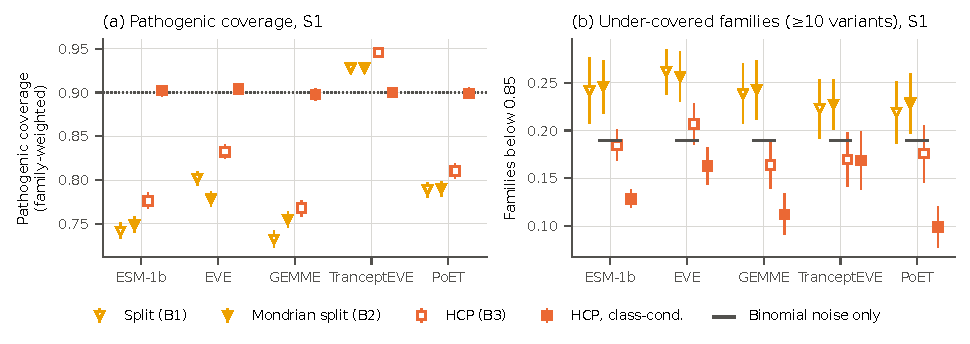
\includegraphics[width=\textwidth]{../figures/fig1_s1_family_coverage.pdf}
\caption{Exchangeable families (S1, $\alpha=0.1$). (a) Family-weighted pathogenic coverage $\Cov_1$ with 95\% family-bootstrap intervals; the dotted line is the target. (b) Fraction of families with at least ten variants whose overall coverage (both classes, for every method) is below 0.85 (mean and s.d. over seeds); the gray dash is the expected fraction if every family had coverage exactly 0.90.}
\label{fig:s1}
\end{figure}

\paragraph{Variant-level calibration misses pathogenic variants per family.}
In S1 (Fig.~\ref{fig:s1}), variant-level split conformal has variant-weighted coverage \sOneBoneCovVar{}, close to its target, but family-weighted coverage \sOneBoneCovFam{}; family-level HCP restores \sOneHcpCovFam{}. The gap is concentrated in the pathogenic class: B2, calibrated class by class over variants, attains variant-weighted pathogenic coverage \sOneBtwoPathVar{} for four predictors yet covers only \sOneBtwoPath{} of pathogenic variants per family. The 5\% of test families with the most pathogenic variants hold \sizeTopShare{} of them, and their pathogenic variants are easier: under B2, families with fewer than five pathogenic variants have pathogenic coverage \sizeCovFew{} against \sizeCovMany{} for families with at least twenty. TranceptEVE is the exception (\sOneBtwoPathTrancept{}), with the error moved to the benign class. Family-level class-conditional calibration attains \sOneHcpccPath{} (pathogenic) and \sOneHcpccBenign{} (benign), as Propositions~\ref{prop:hcp} and~\ref{prop:mondrian} guarantee, and lowers the fraction of under-covered families below the binomial-noise level (Fig.~\ref{fig:s1}b), at the cost of larger sets.

\begin{figure}[t]
\centering
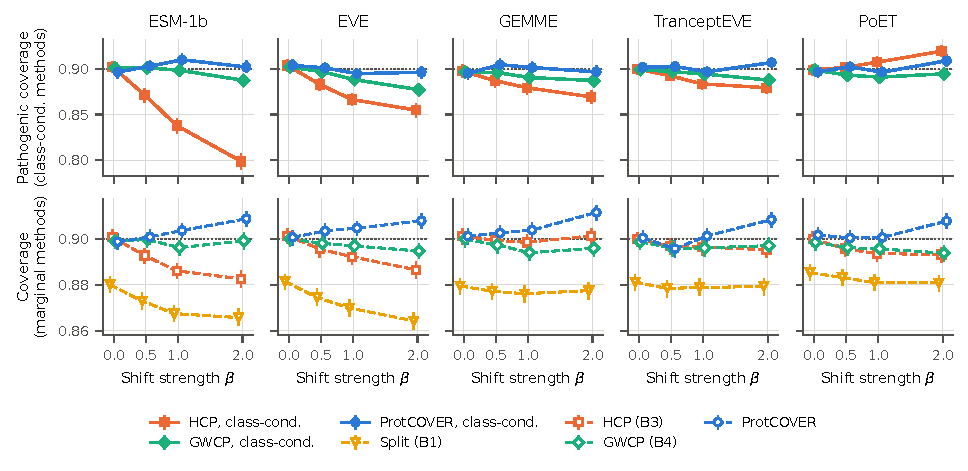
\includegraphics[width=\textwidth]{../figures/fig2_shift_sweep.pdf}
\caption{Coverage under increasing descriptor shift (S2; $\beta=0$ is S1), $\alpha=0.1$, with 95\% family-bootstrap intervals; methods are offset slightly in $\beta$. Top: pathogenic coverage $\Cov_1$ of class-conditional family-level methods (Mondrian split, far below the target for four predictors, is in Table~\ref{tab:main}). Bottom: family-weighted coverage $\Cov$ of marginal methods.}
\label{fig:shift}
\end{figure}

\begin{table}[t]
\caption{Family-weighted pathogenic / benign coverage ($\Cov_1$ / $\Cov_0$) of class-conditional methods at $\alpha=0.1$ (target 0.90), mean over ten seeds. The ProtCOVER row omits the gate, which can only raise coverage (Lemma~\ref{lem:enlarge}); the full method is in Table~\ref{tab:ablation}. Paired differences with intervals are in Table~\ref{tab:paired}.}
\label{tab:main}
\centering\scriptsize\setlength{\tabcolsep}{3pt}
\begin{tabular}{llccccc}
\toprule
Setting & Method & ESM-1b & EVE & GEMME & TranceptEVE & PoET \\
\midrule
S1 (exchangeable) & Mondrian split (B2) & 0.749 / 0.899 & 0.778 / 0.898 & 0.755 / 0.895 & 0.928 / 0.837 & 0.790 / 0.877 \\
 & HCP (B3) & 0.903 / 0.903 & 0.904 / 0.901 & 0.898 / 0.898 & 0.900 / 0.901 & 0.899 / 0.903 \\
 & GWCP (B4) & 0.902 / 0.901 & 0.902 / 0.899 & 0.897 / 0.897 & 0.900 / 0.900 & 0.899 / 0.901 \\
 & ProtCOVER & \textbf{0.897 / 0.904} & \textbf{0.904 / 0.902} & \textbf{0.895 / 0.899} & \textbf{0.902 / 0.902} & \textbf{0.897 / 0.906} \\
\midrule
S2, $\beta=1$ & Mondrian split (B2) & 0.655 / 0.929 & 0.709 / 0.915 & 0.712 / 0.906 & 0.920 / 0.839 & 0.795 / 0.856 \\
 & HCP (B3) & 0.838 / 0.927 & 0.867 / 0.916 & 0.879 / 0.909 & 0.884 / 0.894 & 0.908 / 0.875 \\
 & GWCP (B4) & 0.899 / 0.904 & 0.888 / 0.909 & 0.891 / 0.904 & 0.895 / 0.894 & 0.891 / 0.897 \\
 & ProtCOVER & \textbf{0.910 / 0.905} & \textbf{0.895 / 0.909} & \textbf{0.902 / 0.908} & \textbf{0.897 / 0.898} & \textbf{0.897 / 0.905} \\
\midrule
S2, $\beta=2$ & Mondrian split (B2) & 0.619 / 0.941 & 0.686 / 0.917 & 0.700 / 0.910 & 0.921 / 0.839 & 0.806 / 0.840 \\
 & HCP (B3) & 0.798 / 0.939 & 0.855 / 0.917 & 0.869 / 0.914 & 0.880 / 0.891 & 0.920 / 0.853 \\
 & GWCP (B4) & 0.888 / 0.905 & 0.877 / 0.906 & 0.887 / 0.897 & 0.888 / 0.889 & 0.895 / 0.873 \\
 & ProtCOVER & \textbf{0.902 / 0.915} & \textbf{0.896 / 0.916} & \textbf{0.898 / 0.915} & \textbf{0.908 / 0.900} & \textbf{0.910 / 0.892} \\
\midrule
S3 (orphan families) & Mondrian split (B2) & 0.678 / 0.915 & 0.772 / 0.895 & 0.724 / 0.903 & 0.943 / 0.823 & 0.817 / 0.854 \\
 & HCP (B3) & 0.876 / 0.908 & 0.909 / 0.899 & 0.890 / 0.905 & 0.914 / 0.892 & 0.931 / 0.879 \\
 & GWCP (B4) & 0.889 / 0.905 & 0.903 / 0.898 & 0.895 / 0.900 & 0.903 / 0.913 & 0.901 / 0.900 \\
 & ProtCOVER & \textbf{0.894 / 0.908} & \textbf{0.907 / 0.901} & \textbf{0.900 / 0.908} & \textbf{0.900 / 0.921} & \textbf{0.901 / 0.910} \\
\bottomrule
\end{tabular}

\end{table}

\paragraph{Weighting restores coverage under family-level shift.}
Under S2 (Fig.~\ref{fig:shift}, Table~\ref{tab:main}), family-level calibration alone degrades as $\beta$ grows: at $\beta=1$ its pathogenic coverage spans \sTwoBoneHcpPath{} across predictors, and for ESM-1b it falls to \sTwoBtwoHcpPathEsm{} at $\beta=2$. Its error is not one-sided: for PoET, and for TranceptEVE in S3, it over-covers pathogenic variants while under-covering benign ones. We therefore score each method by the shortfall of its worse class below the target. Over the \nShiftCells{} shifted predictor-setting cells (S2 with $\beta>0$, S3, and S4), this shortfall averages \shortHcpMean{} for HCP (maximum \shortHcpMax{}; worse class below 0.89 in \shortHcpN{} cells), \shortGwcpMean{} for GWCP (\shortGwcpMax{}; \shortGwcpN{} cells), and \shortPwMean{} for ProtCOVER (\shortPwMax{}; \shortPwN{} cells). Both components matter: the same weights applied to variant-level calibration leave a mean shortfall of \shortVarWMean{} (Table~\ref{tab:ablation}). GWCP, whose bins use the two descriptors that define the S2 shift, is the strongest baseline; at $\beta=2$ ProtCOVER's pathogenic coverage exceeds it by \sTwoBtwoDiffGwcp{} with paired intervals above zero for \sTwoBtwoDiffGwcpNpos{} of 5 predictors (Appendix Table~\ref{tab:paired}). S2 favors weighting by construction, since it shifts the very descriptors that $\hat w$ models. On the natural shift of S3, ProtCOVER only matches GWCP (differences \sThreeDiffGwcp{}), while still correcting HCP's errors in both directions. On held-out regions of embedding space (S4), variant-level Mondrian calibration again covers only \sFourBtwoPathNT{} of pathogenic variants per family for four predictors, but family-level calibration alone is already close to the target (worse-class shortfall \shortHcpFourMean{}, maximum \shortHcpFourMax{}), and weighting brings no gain: ProtCOVER's shortfall is \shortPwFourMean{} (maximum \shortPwFourMax{}) against \shortGwcpFourMean{} for GWCP. With little bias left to correct, the estimated weights mainly add variance; in S4, looser clipping lowers coverage (Table~\ref{tab:ablation}). The fraction of under-covered families is similar for the three family-level methods under shift (ProtCOVER \underPwShift{}, GWCP \underGwcpShift{}, HCP \underHcpShift{}; binomial-noise reference \underNullShift{}). Our bootstrap intervals are conditional on the splits; across seeds, ProtCOVER's pathogenic coverage in a cell has standard deviation \seedSdPwPath{}, so differences of about 0.01 between methods should be read with care. The price is larger sets (Fig.~\ref{fig:tradeoff}): averaged over the shifted cells, mean set size is \sizePwShift{} for ProtCOVER, \sizeGwcpShift{} for GWCP and \sizeHcpShift{} for HCP, and ProtCOVER returns both labels for \fullPwRange{} of variants, depending on predictor and setting. At matched pathogenic coverage of 0.90, interpolated along the $\alpha$ curves, the three methods need the same mean set size (\sizeMatchedPw{}, \sizeMatchedGwcp{} and \sizeMatchedHcp{} over the \nMatched{} cells where all three reach 0.90), and paired differences in singleton error at $\alpha=0.1$ are small and of both signs (\diffSingErrGwcp{} against GWCP; Appendix Table~\ref{tab:efficiency}). The extra size thus buys coverage along a shared coverage-size trade-off; it neither costs nor gains efficiency.

\begin{figure}[t]
\centering
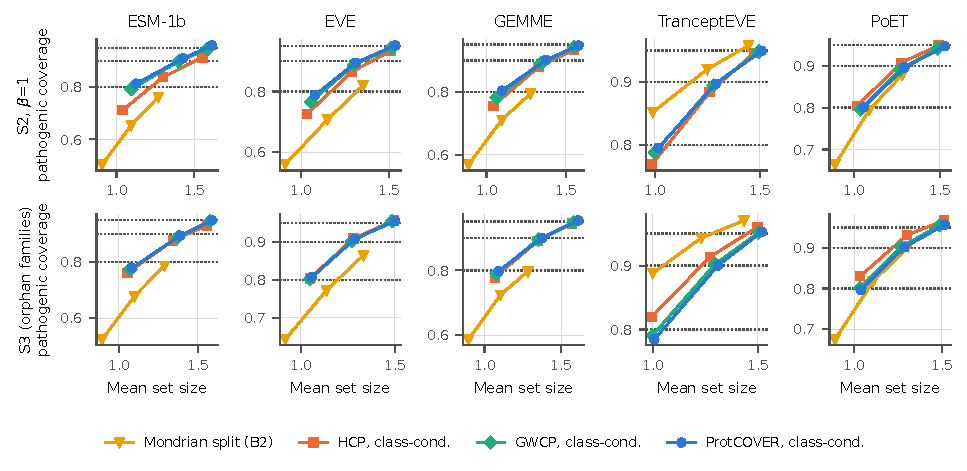
\includegraphics[width=\textwidth]{../figures/fig3_coverage_size.pdf}
\caption{Pathogenic coverage against mean set size for $\alpha\in\{0.2,0.1,0.05\}$ (left to right along each curve), class-conditional methods. Dotted lines mark the three targets.}
\label{fig:tradeoff}
\end{figure}

\paragraph{Summary across shifts.}
Under the natural shifts, family-level calibration does most of the work and weighting is neutral: ProtCOVER minus GWCP in pathogenic coverage spans \sThreeDiffGwcp{} in S3 and \sFourDiffGwcp{} in S4. Under descriptor shift (S2), weighting adds a clear gain with paired intervals above zero. Differences below about 0.01 are within seed-to-seed variation, and since all seeds resplit one pool of families, these conclusions are limited to this benchmark.

\paragraph{The support gate preserves coverage but does not improve selective risk.}
With $(m,\pi_{\max})$ and the kernel scale tuned on training families under a 10\% budget, the gate abstained on at most \gateAbsMaxNoBtwo{} of test families except at $\beta=2$ (\gateAbsBtwo{}), so the full method matches (i)+(ii) (Table~\ref{tab:ablation}). The 10\% budget is a cap: tuning chose so little abstention because abstaining more did not raise retained coverage on the inner split. Risk-coverage curves (Appendix Fig.~\ref{fig:risk}) evaluate the ranking itself at every abstention level, against random abstention averaged over 100 random family orders. Abstaining first on the families with the lowest ESS gave a lower AURC than random abstention in the majority of seeds in \riskEssNBetter{} of \riskNCells{} predictor-setting cells and a higher one in \riskEssNWorse{} (the rest tied); ranking by maximum identity (\riskSupportNBetter{} lower, \riskSupportNWorse{} higher) or by test-point mass (\riskMassNBetter{} lower, \riskMassNWorse{} higher) did no better. On this benchmark, how well a family is supported by calibration data does not predict how often the predictor errs on it once coverage is controlled. The gate therefore adds nothing measurable here; Lemma~\ref{lem:enlarge} guarantees only that it costs no coverage.


\begin{table}[t]
\caption{Ablations: pathogenic coverage $\Cov_1$ at $\alpha=0.1$, mean (minimum) over the five predictors. For family definitions, HCP / ProtCOVER.}
\label{tab:ablation}
\centering\scriptsize\setlength{\tabcolsep}{3pt}
\begin{tabular}{lcccc}
\toprule
Configuration & S2, $\beta=1$ & S2, $\beta=2$ & S3 & S4 \\
\midrule
\multicolumn{5}{l}{\emph{Components}} \\
(i) family-level calibration (HCP) & 0.875 (0.838) & 0.864 (0.798) & 0.904 (0.876) & 0.904 (0.891) \\
(i)+(ii), conditional on $\hat w$ (ProtCOVER) & 0.901 (0.897) & 0.925 (0.920) & 0.902 (0.890) & 0.914 (0.912) \\
(i)+(ii), conditional on descriptors (ProtCOVER-D) & 0.901 (0.898) & 0.902 (0.890) & 0.905 (0.894) & 0.902 (0.885) \\
(i)+(ii), reweighting by $\hat w$ (ProtCOVER-W) & 0.900 (0.895) & 0.902 (0.896) & 0.900 (0.894) & 0.895 (0.886) \\
(i)+(iii) gate & 0.875 (0.838) & 0.864 (0.798) & 0.904 (0.876) & 0.904 (0.891) \\
ProtCOVER-W + (iii) gate & 0.900 (0.895) & 0.904 (0.898) & 0.901 (0.894) & 0.895 (0.886) \\
(ii) without (i): variant-level weighting & 0.789 (0.740) & 0.787 (0.723) & 0.807 (0.740) & 0.798 (0.737) \\
\multicolumn{5}{l}{\emph{Descriptors for $\hat w$ (ProtCOVER-W)}} \\
sequence similarity only & 0.871 (0.850) & 0.853 (0.799) & 0.899 (0.892) & 0.906 (0.903) \\
alignment depth only & 0.899 (0.892) & 0.901 (0.872) & 0.899 (0.878) & 0.903 (0.893) \\
embedding distance only & 0.879 (0.845) & 0.866 (0.806) & 0.904 (0.872) & 0.895 (0.882) \\
the three support groups & 0.900 (0.894) & 0.904 (0.898) & 0.900 (0.894) & 0.896 (0.887) \\
main set + predictor score summaries & 0.903 (0.894) & 0.898 (0.889) & 0.902 (0.895) & 0.894 (0.887) \\
\multicolumn{5}{l}{\emph{Weight clipping $c$ (default 20; ProtCOVER-W)}} \\
$c=5$ & 0.899 (0.894) & 0.889 (0.870) & 0.900 (0.892) & 0.904 (0.897) \\
$c=100$ & 0.900 (0.895) & 0.908 (0.904) & 0.901 (0.894) & 0.883 (0.874) \\
no clipping & 0.900 (0.895) & 0.908 (0.904) & 0.901 (0.894) & 0.837 (0.779) \\
\bottomrule
\end{tabular}

\end{table}

\paragraph{Ablations.}
Table~\ref{tab:ablation} shows that sequence similarity or embedding distance alone does not correct the S2 shift, alignment depth alone helps on average but not for every predictor, and the support descriptors together match the full set; adding the predictor's score summaries does not help and lowers the worst predictor's coverage at $\beta=2$. Embedding distance contributes little here because it barely differs between calibration and test families (mean \sTwoCalEmb{} against \sTwoTestEmb{} at $\beta=1$). Tight clipping ($c=5$) under-corrects at $\beta=2$, while loose or no clipping hurts in S4, so the clipping level trades bias correction against variance. Under the alternative family definitions, ProtCOVER's mean pathogenic coverage over predictors stays at \sensPwMeanRange{} across the shifted settings; its worst predictor-setting cell is \sensFiftyPwMin{} with 50\% clustering and \sensHcPwMin{} with homology components, against \sensFiftyHcpMin{} and \sensHcHcpMin{} for HCP.

\paragraph{Deployment-realistic features.}
The base model's within-protein standardization and the variant-count descriptor both need the query protein's whole variant panel. Without them (raw score only, no variant count; Table~\ref{tab:ablation}), Mondrian split still covers only \realBtwoPath{} of pathogenic variants per family in S1, below the target for \realBtwoNBelow{} of 5 predictors, and the ranking under shift is unchanged: mean worse-class shortfall \realShortPwMean{} for ProtCOVER, \realShortGwcpMean{} for GWCP and \realShortHcpMean{} for HCP (worst coverage \realWorstPw{}, \realWorstGwcp{} and \realWorstHcp{}). Sets are smaller for every method, for example \realSizePw{} for ProtCOVER against \sizePwShift{} with the full features.

\subsection{Synthetic validation}\label{sec:synthetic}
On simulated families where A1 or A2 hold exactly (Appendix~\ref{app:synthetic}), family-weighted coverage at a 0.90 target is \synHcpEasy{} for family-level and \synBoneEasy{} for variant-level calibration, and under a strong family-level shift ($\beta=2$) weighting with cross-fitted estimated ratios attains \synShiftTwoEst{} where family-level calibration alone falls to \synShiftTwoHcp{}.

\section{Limitations}\label{sec:limitations}

\emph{What the guarantees assume.} Exact coverage needs exchangeable families (A1), or a family-level shift whose density ratio is a nonnegative function in the span of the features; with an estimated ratio it needs the ratio to be fitted on families independent of those it calibrates (Lemma~\ref{lem:crossfit}), and the class-conditional versions hold for families that contain the class. Every guarantee is marginal over families: ProtCOVER certifies no particular protein, and the coverage of a small family is dominated by binomial noise. Under any other shift, Corollary~\ref{cor:conditional} bounds the loss by total-variation distances that cannot be estimated from unlabeled data, and when a family's scores and labels given its descriptors differ between calibration and deployment (A2 fails, as in S5), every method under-covers and the ratio gives no warning.

\emph{What is only measured.} The comparison with the baselines, the robustness to the family definition, the base model and missing alignments, and the external results are empirical. Beyond the 0.01 margin, ProtCOVER's advantage over group-weighted conformal prediction is confined to descriptor shift (S2) on one benchmark whose ten seeds resplit one pool of families; on orphan families, held-out embedding regions and the external evaluations it matches group weighting. The advantage is in coverage, not efficiency: ProtCOVER buys its smaller shortfall with larger sets under shift.

\emph{Scope.} The ratio-based version needs a batch of unlabeled target families, or a reference panel such as the unlabeled proteome for a single query; ProtCOVER-D does not, at a somewhat larger shortfall. The base model is deliberately simple, and a stronger one may give smaller sets. ProtCOVER outputs prediction sets, not ACMG/AMP evidence strengths; mapping sets to PP3/BP4 strengths is future work.

\section{Conclusion}\label{sec:conclusion}

Calibrating a variant effect predictor variant by variant lets well-studied families set its error rate: on ProteinGym, Mondrian split conformal covers only \sOneBtwoPath{} of pathogenic variants per family for four of five predictors, without any shift. Treating families as the exchangeable unit removes this failure, and conditioning a family-weighted quantile regression on a cross-fitted density ratio keeps coverage exact both under family exchangeability and under the estimated shift. The empirical gain is specific to descriptor shift. Under it (S2), ProtCOVER's mean worse-class shortfall is \shortCrTwoMean{}, against \shortGwcpTwoMean{} for group weighting and \shortHcpTwoMean{} for HCP; on orphan families and held-out embedding regions it matches group weighting (\shortCrIndMean{} against \shortGwcpIndMean{}). The gain is in coverage, not in set size, and a shift in predictor accuracy that the descriptors do not encode defeats every label-free method.


\FloatBarrier % place every figure and table of the main text before the references
\section*{Code Availability}
Code and scripts that regenerate every number, table and figure from the public ProteinGym release: \url{https://github.com/wael-fahmy/protcover} (MIT license).

\bibliographystyle{splncs04}
\bibliography{refs}

\appendix
\section{Proofs}\label{app:proofs}

Throughout, $F_k=N_k^{-1}\sum_{i=1}^{N_k}\delta_{S_{k,i}}$ is the score distribution of family $k$ (for the test family it involves unobserved labels and is used only in the analysis), and $\gamma_{K+1}(C)=F_{K+1}((-\infty,\hat q])$ because a test variant is covered iff its score is at most $\hat q$.

\paragraph{Comparison step for~\eqref{eq:threshold}.}
Fix weights $p_1,\dots,p_{K+1}$ and define the oracle measure $\mu=\sum_{k=1}^{K+1}p_kF_k$ and $q=\Qt_{1-\alpha}(\mu)$. The computable $\hat\mu$ moves the mass $p_{K+1}$ from $F_{K+1}$ to $+\infty$, so $\hat\mu((-\infty,u])\le\mu((-\infty,u])$ for every $u$, hence $\hat q\ge q$ and $\gamma_{K+1}(C)\ge F_{K+1}((-\infty,q])$. Also $\mu((-\infty,q])\ge1-\alpha$ by right-continuity.

\begin{proof}[Proposition~\ref{prop:hcp}]
With $\omega\equiv1$, $p_k=1/(K+1)$ and $q$ is a symmetric function of $(G_1,\dots,G_{K+1})$. By exchangeability, $\E[F_{K+1}((-\infty,q])]=\E[(K+1)^{-1}\sum_kF_k((-\infty,q])]=\E[\mu((-\infty,q])]\ge1-\alpha$, and the comparison step gives $\Cov(C)\ge1-\alpha$.
\end{proof}

\begin{proof}[Theorem~\ref{thm:conditional}]
Let $L^o(b)=\sum_{k=1}^{K+1}N_k^{-1}\sum_i\rho_\tau(S_{k,i}-\Phi(D_k)^\top b)$ be the oracle objective, in which the test family enters with its true scores. It is convex, piecewise linear and nonnegative, so its minimizers form a nonempty closed convex polyhedron; let $\tilde b$ be the one of minimum Euclidean norm (a measurable function of the data, for example as the limit of the ridge-penalized minimizers as the penalty vanishes; only its symmetry is used), $\tilde g=\Phi^\top\tilde b$, and $\tilde\gamma_k=N_k^{-1}\sum_i\1\{S_{k,i}\le\tilde g(D_k)\}$.

\emph{(a) First-order condition.} Let $f=\Phi^\top b_f$ with $f(D)\ge0$ $P$-a.s.; then $f(D_k)\ge0$ for every $k$ almost surely, which is all the argument uses. The right derivative of $t\mapsto\rho_\tau(S-\tilde g(D)-tf(D))$ at $t=0$ is $f(D)(\1\{S\le\tilde g(D)\}-\tau)$ (if $S=\tilde g(D)$, the residual is $-tf(D)\le0$ for $t>0$). The right derivative of $t\mapsto L^o(\tilde b+tb_f)$ at $0$ is therefore $\sum_{k=1}^{K+1}f(D_k)(\tilde\gamma_k-\tau)$, which is nonnegative at a minimizer.

\emph{(b) Symmetry.} $L^o$, and hence $\tilde b$, is invariant to permutations of the families, so the pairs $(f(D_k),\tilde\gamma_k)$, $k\le K+1$, are exchangeable under $P^{K+1}$ and $\E_{P^{K+1}}[f(D_{K+1})(\tilde\gamma_{K+1}-\tau)]=(K+1)^{-1}\E\sum_kf(D_k)(\tilde\gamma_k-\tau)\ge0$; the expectation exists because $\tilde\gamma\in[0,1]$ and $\E_Pf<\infty$.

\emph{(c) Change of measure.} For any bounded measurable $H$ of the families, $\E_{P^{K+1}}[f(D_{K+1})H]=\E_Pf(D)\cdot\E_{P^K\times Q_f}[H]$. With $H=\tilde\gamma_{K+1}-\tau$, (b) gives $\E_{P^K\times Q_f}[\tilde\gamma_{K+1}]\ge\tau$.

\emph{(d) The computable threshold dominates the oracle.} We show $\hat q\ge\tilde g(D_{K+1})$, which gives $\gamma_{K+1}(C)\ge\tilde\gamma_{K+1}$ and, with (c), the theorem. The argument follows Proposition~6 of~\cite{gibbs2025conformal} (imputing an upper bound $M$), with the supremum over the solution set in place of a min-norm solution, and $M\to\infty$. Write $\phi_t=\Phi(D_{K+1})$. If $L$ in~\eqref{eq:condcal} is unbounded below, $\hat q=+\infty$. Otherwise $A=\arg\min L$ is nonempty (a polyhedral function bounded below attains its minimum). Pick $M$ larger than every test score and than $\inf_{b\in A}\phi_t^\top b$, and let $L^M$ be $L^o$ with every test score replaced by $M$. Since $\rho_\tau(u)\ge\tau u$ with equality for $u\ge0$, $L^M(b)=L(b)+\tau\phi_t^\top b+\rho_\tau(M-\phi_t^\top b)\ge L(b)+\tau M$, with equality when $\phi_t^\top b\le M$, which holds for some $b\in A$; hence $\min L^M=\min L+\tau M$ and $\arg\min L^M\subseteq A$. Let $b'\in\arg\min L^M$, $a=\tilde g(D_{K+1})$ and $a'=\phi_t^\top b'$. Adding $L^o(\tilde b)\le L^o(b')$ and $L^M(b')\le L^M(\tilde b)$, the calibration terms cancel and $\sum_i[h_i(a)-h_i(a')]\le0$, where $h_i(c)=\rho_\tau(S_{K+1,i}-c)-\rho_\tau(M-c)$ is nondecreasing in $c$ because $S_{K+1,i}\le M$ and $\rho_\tau$ is convex. If $a'<a$, then $h_i(a')\le h_i(a)$ for every $i$, so both optimality inequalities hold with equality and $\tilde b\in\arg\min L^M\subseteq A$. In either case $\hat q=\sup_{b\in A}\phi_t^\top b\ge a$.

The case $f\equiv1$ gives the statement under A1 (for exchangeable rather than i.i.d.\ families, (b) applies directly with $f\equiv1$).
\end{proof}

\paragraph{Computing the supremum.}
Let $L'$ be $L$ with the test term's weight raised from $\tau$ to $\tau'>\tau$, so $L'(b)=L(b)-(\tau'-\tau)\phi_t^\top b$. If $b\in\arg\min L$ and $b'\in\arg\min L'$, adding $L(b)\le L(b')$ and $L'(b')\le L'(b)$ gives $(\tau'-\tau)\,\phi_t^\top(b'-b)\ge0$, so every minimizer of $L'$ has $\phi_t^\top b'\ge\hat q$. If $L$ is unbounded below along a direction $d$, its recession slope along $d$ is negative, which forces $\phi_t^\top d>0$, so $L'$ is unbounded along $d$ as well. If $L$ is bounded but $\hat q=+\infty$, then $A$ contains points with $\phi_t^\top b\to\infty$ and $L'$ is unbounded below on $A$. In every case the threshold computed with $\tau'=\tau+10^{-4}$ (the perturbed program's optimal fitted value, or $+\infty$ when its dual is infeasible) is at least $\hat q$; it equals $\hat q$ when $\tau'-\tau$ is small enough for the data (the optimal value is concave and piecewise linear in $\tau'$, with finitely many breakpoints, and its right derivative at $\tau$ is $-\hat q$), and is otherwise conservative. Appendix~\ref{app:protocol} checks the computed thresholds against an independent computation under solver tolerances. By Lemma~\ref{lem:enlarge} the computed sets keep every guarantee. Standardizing the descriptors (ProtCOVER-D) is an invertible affine reparametrization of $b$ that does not change $\mathcal{F}$, so fitted values, and $\hat q$, are unchanged.

\begin{proof}[Corollary~\ref{cor:conditional}]
Let $\phi(g)\in[0,1]$ be the expected per-family coverage of a test family $g$ over $G_1,\dots,G_K\sim P$. For $f\in\mathcal{F}$, $f\ge0$, Theorem~\ref{thm:conditional} gives $\E_{Q_f}\phi\ge1-\alpha$, and $|\E_Q\phi-\E_{Q_f}\phi|\le\dtv(Q,Q_f)$. For $\Phi=(1,\hat w)$, condition on $\hat w$: $f\equiv1$ and $f=\hat w$ are nonnegative members of $\mathcal{F}$ with $Q_1=P$ and $Q_{\hat w}=\hat Q$.
\end{proof}

\begin{proof}[Proposition~\ref{prop:weighted}]
Under A2 the joint law of $(G_1,\dots,G_{K+1})$ has density $\prod_{k\le K}\pi(g_k)\cdot w(d_{K+1})\pi(g_{K+1})$ with respect to a product base measure, where $\pi$ is a density of $P$, so the sequence is weighted exchangeable with weight functions $1,\dots,1,w$~\cite[Def.~1, Lemma~2]{tibshirani2019conformal}. Let $E$ be the event that the unordered collection $\{G_1,\dots,G_{K+1}\}$ equals $\{g_1,\dots,g_{K+1}\}$. As in the proof of Lemma~3 of~\cite{tibshirani2019conformal}, $\P(G_{K+1}=g_k\mid E)=w(d_k)/\sum_jw(d_j)=p_k$ (summing over coincident values). The $p_k$, $\mu$ and $q$ are functions of $E$, so $\E[F_{K+1}((-\infty,q])\mid E]=\mu((-\infty,q])\ge1-\alpha$, and the comparison step gives the first claim. For $\hat w$ independent of the families, the procedure is invariant to rescaling the weights, so conditionally on $\hat w$ it is the procedure of the first claim for the shift $\hat Q$; the total-variation argument of Corollary~\ref{cor:conditional} gives the second claim.
\end{proof}

\begin{proof}[Lemma~\ref{lem:crossfit}]
The ratio for fold $j$ is fitted on the fitting calibration families and the target families outside fold $j$, rescaled to mean one over the fitting calibration families and clipped by a fixed rule; no other family enters it. Under A2 all families are mutually independent, so $\hat w_j$ is independent of the calibration families used in~\eqref{eq:threshold} and~\eqref{eq:condcal} and of each family of fold $j$, which, conditionally on $\hat w_j$, are still i.i.d.\ $P$ and $Q$. Each query family of fold $j$ plays the role of $G_{K+1}$ in Corollary~\ref{cor:conditional} and Proposition~\ref{prop:weighted}. If the non-training families are exchangeable (a random split of an exchangeable pool, given the training families), then conditionally on the multiset of families that fit $\hat w_j$, the other calibration families together with any one family of fold $j$ are exchangeable, and $\hat w_j$, hence $\Phi$, is fixed; step (b) of the proof of Theorem~\ref{thm:conditional} with $f\equiv1$ applies directly to them, and (d) is unchanged. A unit test in the released code checks that a family's weight does not change when the other calibration families change.
\end{proof}

\begin{proof}[Proposition~\ref{prop:mondrian}]
Fix $y$ and let $\mathcal{I}_y=\{k\le K+1:N_{k,y}>0\}$. Conditionally on $\mathcal{I}_y$, with $K+1\in\mathcal{I}_y$, the families indexed by $\mathcal{I}_y$ are exchangeable under A1 (the event $\{\mathcal{I}_y=I\}$ is invariant under permutations of $I$) and independent in the other settings, with laws $P_y=P(\cdot\mid N_y>0)$ for calibration families and the test law conditioned on $N_y>0$. Because $\1\{N_y>0\}$ is a function of $G$, a test law with density $f(D)/\E_Pf$ with respect to $P$ has, after conditioning, density proportional to $f(D)$ with respect to $P_y$. The label-$y$ procedures are the procedures above applied to these families with $F_k$ replaced by the label-$y$ score distribution $F_k^y$ (weights $1/N_{k,y}$), so every proof applies verbatim, and the normalizing constants cancel.
\end{proof}

\begin{proof}[Lemma~\ref{lem:enlarge}]
$\1\{Y\in C'(X)\}\ge\1\{Y\in C(X)\}$ pointwise, so every average and expectation of the indicators is at least as large for $C'$.
\end{proof}

\section{Protocol Details}\label{app:protocol}

\paragraph{Predictors.} The five unsupervised predictors are all the non-clinical models in ProteinGym v1.3's clinical score files (columns ESM1b, EVE, GEMME, TranceptEVE\_L, PoET; PoET is the 200M model). The other columns are clinical predictors trained or tuned on clinical labels.

\paragraph{Families and homology.} MMseqs2 release 18-8cc5c. Clusters: \texttt{cluster} with minimum identity 0.3 (0.5 for the sensitivity check), coverage 0.8 and coverage mode 0 (both sequences). Homology search: all against all, sensitivity 7.5, $E\le10$, at most 500 hits per query; hits are then filtered at $E\le10^{-3}$. Homology components additionally require identity $\ge0.3$ and coverage $\ge0.5$ of both sequences; the strictest definition takes connected components of all hits with $E\le10^{-3}$ (\nFamRemote{} families, \nFamRemoteSingleton{} single proteins, one component of \maxFamRemote{} proteins).

\paragraph{Descriptors.} Per protein: maximum identity to any training protein over hits with $E\le10^{-3}$ (0 without a hit); $\log(1+N_{\mathrm{eff}})$ with $N_{\mathrm{eff}}$ the sum of ProteinGym's MSA sequence weights; $\log$ of $N_{\mathrm{eff}}$ divided by alignment length; cosine distance of the mean-pooled last-layer (layer 12) embedding of \texttt{esm2\_t12\_35M\_UR50D} to the nearest training protein (sequences over 1022 residues are embedded in windows of 1022 with stride 511 and residue representations averaged over windows); $\log$ length. Per family: the maximum of maximum identity and the minimum of embedding distance over member proteins, the mean of the other protein descriptors, and $\log$ of the family's number of scored variants. Descriptors are recomputed for every split because they depend on its training families.

\paragraph{Splits.} S2 uses $z$, the mean of the standardized maximum identity and $\log N_{\mathrm{eff}}$ over non-training families, and Efraimidis--Spirakis keys $\log(u)\,e^{\beta z}$ with uniforms $u$ shared across $\beta$, so the sweep is coupled and $\beta=0$ is S1. S3 draws test families uniformly from orphan families and training and calibration families uniformly from the rest. S4 regions are fixed once, before any S4 run: each family's embedding is the mean of its members' unit-normalized ESM2 embeddings, renormalized; after centering, the first 50 principal components are clustered by $k$-means ($k=20$, ten restarts, seed 0). Each seed permutes the regions and adds whole regions to the test set until it holds 30\% of families (the last region is split at random); training and calibration families are drawn uniformly from the remaining families. S4s permutes the regions in the same way but adds a region only if the test set stays within 30\% of families, skipping the others, so that every test region is held out whole (\sFourStrictTestFam{} test families per seed); training and calibration families are drawn uniformly from the remaining families in the proportions 40:30. S5 keeps the S1 training families; $z$ is the standardized mean over the five predictors of each family's within-family AUC (families without both classes get the median), and test families are drawn as in S2 with $\beta=1$. The ten seeds resplit one fixed pool of families, so they are not independent samples of the population of families.

\paragraph{Base model and conformal methods.} The base model standardizes its two features (clipped raw score and the score standardized over the protein's scored variants) and fits $L_2$-regularized logistic regression ($C=1$). Dunn et al.'s repeated subsampling uses 50 subsamples. GWCP uses nine bins: maximum identity zero, at most the median of the positive values, or above it, crossed with $\log N_{\mathrm{eff}}$ terciles over calibration and test families; its target proportions are the bin frequencies over all test families (label-free), and it pools at the family level like HCP. For $\hat w$, one third of the calibration families fit the classifier (logistic regression with ten candidate penalties, five-fold cross-validated log loss) and the test families are split into five folds. ProtCOVER uses the features $(1,\hat w_j)$ on the remaining calibration families for queries of fold $j$; ProtCOVER-D uses an intercept and maximum identity to training, $\log N_{\mathrm{eff}}$, $\log N_{\mathrm{eff}}$ per position and embedding distance, standardized over all calibration families. Both feature classes were fixed in the configuration before the conditional methods were first run. The alignment-free run, with the deployment-realistic base model, removes $\log N_{\mathrm{eff}}$ and $\log N_{\mathrm{eff}}$ per position from the density ratio, from ProtCOVER-D's features and from the gate, and GWCP crosses maximum identity with embedding-distance terciles instead. The linear programs are solved with HiGHS 1.11 (\texttt{highspy}), warm-started across test families, with a cold SciPy solve as fallback.

\paragraph{Threshold audit.} The production code solves the perturbed dual with HiGHS's default feasibility tolerances ($10^{-7}$) and puts a label in the set when its score is at most the threshold plus $10^{-9}$, a guard against rounding that can only enlarge sets (Lemma~\ref{lem:enlarge}). To check that the computed thresholds are conservative under these tolerances, \texttt{scripts/audit\_thresholds.py} recomputes \auditN{} of them independently (ProtCOVER and ProtCOVER-D; seed 0; S1, S2 at $\beta\in\{0.5,1,2\}$, S3 and S4; all five predictors; both classes; three random test families per fold): on the primal program with the exact test weight $\tau$, it minimizes $L$ and then maximizes the query's fitted value subject to $L(b)\le L^\star$, both with tolerances of $10^{-10}$. Every reference computation succeeded, \auditSlack{} of them only after rounding forced a relative slack of $10^{-12}$ on $L^\star$. The two computations agree on whether the threshold is infinite (both are, in \auditBothInf{} cases). The production threshold exceeds the reference by more than $10^{-6}$ in \auditAbove{} cases, by at most \auditMaxDiff{}; there $\tau+10^{-4}$ crosses a breakpoint of the optimal value, because with $\tau+10^{-5}$ or $\tau+10^{-6}$ the same thresholds match the reference to \auditEpsDiff{}. It is below the reference in \auditBelow{} cases, by at most \auditMinDiff{}; these are exactly the cases that needed slack, which can raise the reference's fitted value, so they are within the precision of the check. Elsewhere the two agree to \auditRest{}. No audited test variant changes membership between the two thresholds (\auditLost{} lost, \auditAdded{} added).

\paragraph{External test set.} ClinVar \texttt{variant\_summary} (October 2026) and \texttt{hgvs4variation} map VariationIDs to protein changes in the benchmark's RefSeq proteins; we keep single-nucleotide missense variants on GRCh38 with at least one review star, labeled pathogenic/likely pathogenic or benign/likely benign, whose VariationID is absent from the June 2023 release and whose protein change is not in the benchmark. Excluded as a precaution: VariationIDs present in the July 2023 release and changes that were in the June 2023 release under another VariationID. ESM-1b scores are the precomputed log-likelihood ratios of Brandes et al.~\cite{brandes2023genome}, oriented as in the benchmark; for proteins of at most 1,022 residues they equal the benchmark's to rounding, so only those are used (longer proteins hold \extFracLong{} of the new variants). The build script, the pre-registration and its amendment, and the outcome are in the repository.

\paragraph{Gate.} The gate acts on the family of a query protein, so all variants of that family share one decision. With standardized support descriptors $\tilde d$, the kernel weights $\kappa_{tk}=\exp(-\|\tilde d_k-\tilde d_t\|^2/2b^2)$ give the effective number of calibration families that resemble query family $t$, $\mathrm{ESS}_t=(\sum_k\kappa_{tk})^2/\sum_k\kappa_{tk}^2$, and the test-point mass $\pi_t=p_{K+1}$ of ProtCOVER-W measures how much of the weighted quantile's mass sits on the query itself. The gate abstains when $\mathrm{ESS}_t<m$ or $\pi_t>\pi_{\max}$: the first catches queries with few similar calibration families, the second queries that the ratio marks as far more typical of the targets than of the calibration families. Tuned under the 10\% budget (a cap), it abstained on at most \gateAbsMaxNoBtwo{} of test families except at $\beta=2$ (\gateAbsBtwo{}).

\paragraph{Gate tuning.} An inner split of each seed's training families holds out 40\% as inner training families (descriptors are recomputed relative to them) and draws 30\% as inner test families with the S2 sampler at $\beta=1$; the rest are inner calibration families. Grids: kernel scale $\{0.1,0.2,0.35,0.5,1\}$ times the median pairwise distance of standardized support descriptors, $m\in\{0,2,5,10,20,40\}$, $\pi_{\max}\in\{1,0.05,0.02,0.01,0.005\}$, abstention budget 10\%, coverage tolerance 0.005.

\paragraph{Metrics.} Coverage metrics average per-family coverage over families; set size and singleton rate average over variants. The under-covered fraction uses overall per-family coverage (both classes) for families with at least ten variants, for marginal and class-conditional methods alike; its binomial reference is the expected fraction under $\mathrm{Binomial}(N_k,1-\alpha)$. Bootstrap intervals use 1000 resamples of test families within each seed, holding that seed's calibration draw fixed, so they are conditional on the splits; seed-to-seed variation is reported separately. Random abstention in risk-coverage curves is averaged over 100 random family orders per cell.

\section{Synthetic Validation}\label{app:synthetic}

We simulate families with a descriptor $d\sim N(0,1)$, random offsets, and slopes on the score whose mean depends on $d$, with a fixed base model, so that the truth is known (\synNRep{} replicates, Monte Carlo standard error of every coverage at most \synMaxSe{}). Under A1 with larger families being easier, variant-level split conformal has variant-weighted coverage \synBoneEasyVar{} but family-weighted coverage \synBoneEasy{}, while HCP attains \synHcpEasy{} and single subsampling \synSubEasy{}. Under exact family-level covariate shift (A2, test descriptors $N(-\beta,1)$), HCP drops to \synShiftOneHcp{} at $\beta=1$ and \synShiftTwoHcp{} at $\beta=2$; weighting with the true ratio attains \synShiftOneOracle{} and \synShiftTwoOracle{}, and with cross-fitted estimated ratios \synShiftOneEst{} and \synShiftTwoEst{} (class-conditional pathogenic: \synShiftOneEstCc{} and \synShiftTwoEstCc{}). The excess at $\beta=2$ is the price of the test-point mass, which grows when few calibration families resemble the test family.

For the class-conditional versions we report the worse of the two class-wise coverages (target 0.90). Under the Gaussian shift at $\beta=1$ and $\beta=2$, it is \synShiftOneHcpWorse{} and \synShiftTwoHcpWorse{} for HCP; conditional calibration on $(1,w)$ with the true ratio, the case Theorem~\ref{thm:conditional} covers exactly, attains \synShiftOneCoWorse{} and \synShiftTwoCoWorse{}; ProtCOVER, with the cross-fitted ratio, \synShiftOneCrWorse{} and \synShiftTwoCrWorse{}; ProtCOVER-D, whose features $(1,d)$ do not span this ratio, \synShiftOneCsWorse{} and \synShiftTwoCsWorse{}; and reweighting with the true ratio \synShiftOnePwoWorse{} and \synShiftTwoPwoWorse{}. To test the theorem where the descriptor features are exact, a second shift draws calibration descriptors from $U(-2,2)$ and test descriptors with density $(2-d)/8$ on $[-2,2]$, so that $w(d)=(2-d)/2$ is affine in $d$: HCP attains \synLinHcpWorse{}, and ProtCOVER-D \synLinCsWorse{}, conditional calibration on the true ratio \synLinCoWorse{}, ProtCOVER \synLinCrWorse{} and reweighting with the true ratio \synLinPwoWorse{}. The central checks are also unit tests in the released code.

\section{Additional Results}\label{app:tables}

\begin{figure}[h]
\centering
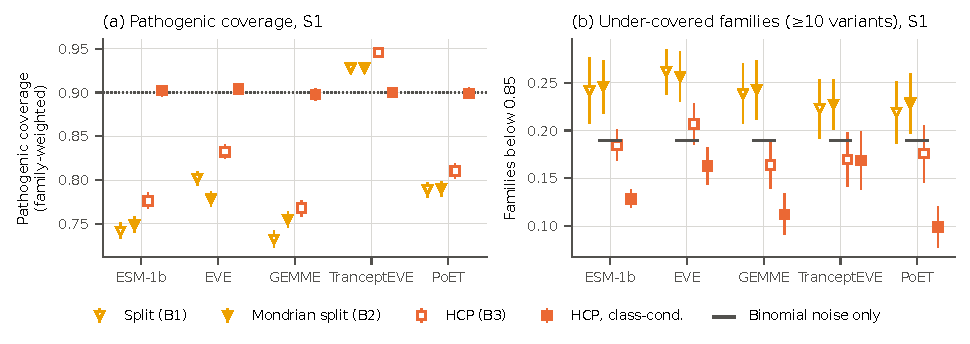
\includegraphics[width=\textwidth]{../figures/fig1_s1_family_coverage.pdf}
\caption{Exchangeable families (S1, $\alpha=0.1$). (a) Family-weighted pathogenic coverage $\Cov_1$ with 95\% family-bootstrap intervals; the dotted line is the target. (b) Fraction of families with at least ten variants whose coverage is below 0.85 (mean and s.d.\ over seeds); the gray dash is the expected fraction if every family had coverage exactly 0.90.}
\label{fig:s1}
\end{figure}

\begin{figure}[h]
\centering
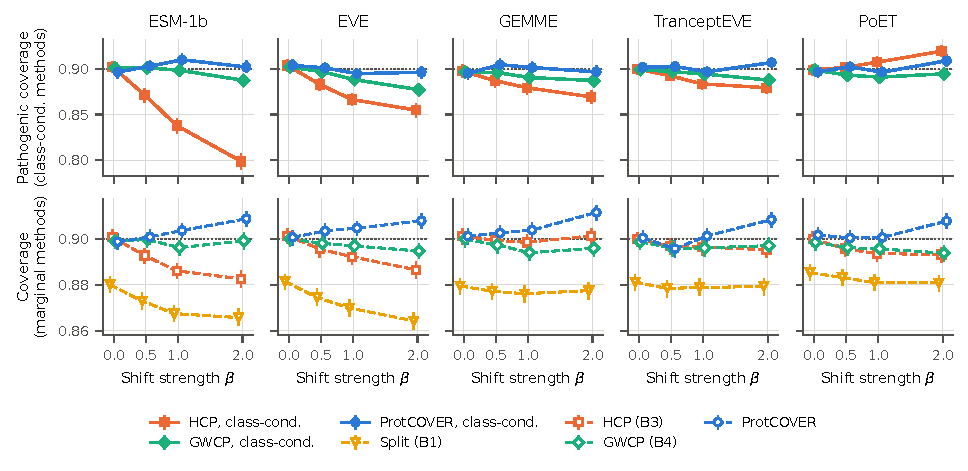
\includegraphics[width=\textwidth]{../figures/fig2_shift_sweep.pdf}
\caption{Class-conditional coverage of both classes under increasing descriptor shift (S2; $\beta=0$ is S1), $\alpha=0.1$, with 95\% family-bootstrap intervals; methods are offset slightly in $\beta$. Mondrian split conformal, far below target, is omitted (Fig.~\ref{fig:s1}).}
\label{fig:shift}
\end{figure}

\begin{figure}[h]
\centering
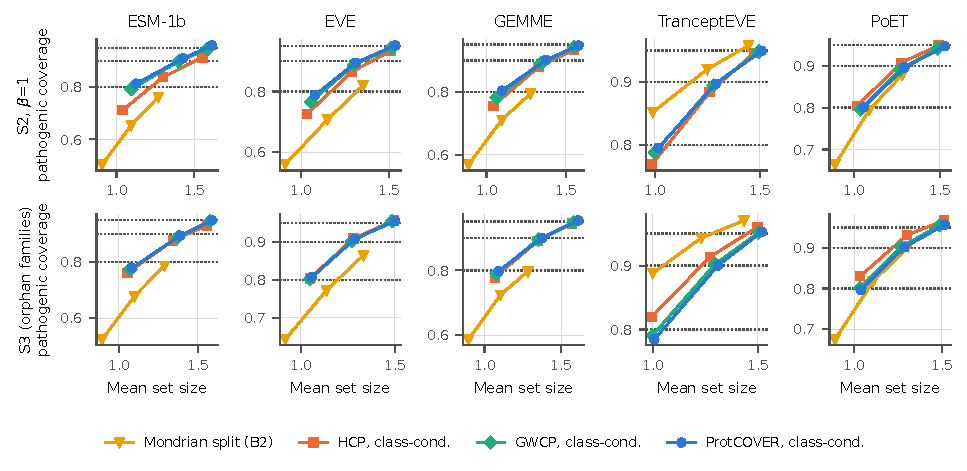
\includegraphics[width=\textwidth]{../figures/fig3_coverage_size.pdf}
\caption{Pathogenic coverage against mean set size for $\alpha\in\{0.2,0.1,0.05\}$ (left to right along each curve), class-conditional methods, on the two shifts defined independently of the descriptors. Dotted lines mark the three targets. A short vertical bar on the 0.90 line marks where a method's curve crosses pathogenic coverage 0.90, found by linear interpolation between its two neighboring levels: the set size the method needs for that coverage, the quantity compared in the last row of Table~\ref{tab:summary}. The methods lie on one coverage-size curve, so a method that covers more also returns larger sets.}
\label{fig:tradeoff}
\end{figure}

\begin{table}[h]
\caption{Family-weighted pathogenic / benign coverage ($\Cov_1$ / $\Cov_0$) of class-conditional methods at $\alpha=0.1$ (target 0.90), per predictor, mean over ten seeds.}
\label{tab:main}
\centering\scriptsize\setlength{\tabcolsep}{3pt}
\begin{tabular}{llccccc}
\toprule
Setting & Method & ESM-1b & EVE & GEMME & TranceptEVE & PoET \\
\midrule
S1 (exchangeable) & Mondrian split (B2) & 0.749 / 0.899 & 0.778 / 0.898 & 0.755 / 0.895 & 0.928 / 0.837 & 0.790 / 0.877 \\
 & HCP (B3) & 0.903 / 0.903 & 0.904 / 0.901 & 0.898 / 0.898 & 0.900 / 0.901 & 0.899 / 0.903 \\
 & GWCP (B4) & 0.902 / 0.901 & 0.902 / 0.899 & 0.897 / 0.897 & 0.900 / 0.900 & 0.899 / 0.901 \\
 & ProtCOVER & \textbf{0.897 / 0.904} & \textbf{0.904 / 0.902} & \textbf{0.895 / 0.899} & \textbf{0.902 / 0.902} & \textbf{0.897 / 0.906} \\
\midrule
S2, $\beta=1$ & Mondrian split (B2) & 0.655 / 0.929 & 0.709 / 0.915 & 0.712 / 0.906 & 0.920 / 0.839 & 0.795 / 0.856 \\
 & HCP (B3) & 0.838 / 0.927 & 0.867 / 0.916 & 0.879 / 0.909 & 0.884 / 0.894 & 0.908 / 0.875 \\
 & GWCP (B4) & 0.899 / 0.904 & 0.888 / 0.909 & 0.891 / 0.904 & 0.895 / 0.894 & 0.891 / 0.897 \\
 & ProtCOVER & \textbf{0.910 / 0.905} & \textbf{0.895 / 0.909} & \textbf{0.902 / 0.908} & \textbf{0.897 / 0.898} & \textbf{0.897 / 0.905} \\
\midrule
S2, $\beta=2$ & Mondrian split (B2) & 0.619 / 0.941 & 0.686 / 0.917 & 0.700 / 0.910 & 0.921 / 0.839 & 0.806 / 0.840 \\
 & HCP (B3) & 0.798 / 0.939 & 0.855 / 0.917 & 0.869 / 0.914 & 0.880 / 0.891 & 0.920 / 0.853 \\
 & GWCP (B4) & 0.888 / 0.905 & 0.877 / 0.906 & 0.887 / 0.897 & 0.888 / 0.889 & 0.895 / 0.873 \\
 & ProtCOVER & \textbf{0.902 / 0.915} & \textbf{0.896 / 0.916} & \textbf{0.898 / 0.915} & \textbf{0.908 / 0.900} & \textbf{0.910 / 0.892} \\
\midrule
S3 (orphan families) & Mondrian split (B2) & 0.678 / 0.915 & 0.772 / 0.895 & 0.724 / 0.903 & 0.943 / 0.823 & 0.817 / 0.854 \\
 & HCP (B3) & 0.876 / 0.908 & 0.909 / 0.899 & 0.890 / 0.905 & 0.914 / 0.892 & 0.931 / 0.879 \\
 & GWCP (B4) & 0.889 / 0.905 & 0.903 / 0.898 & 0.895 / 0.900 & 0.903 / 0.913 & 0.901 / 0.900 \\
 & ProtCOVER & \textbf{0.894 / 0.908} & \textbf{0.907 / 0.901} & \textbf{0.900 / 0.908} & \textbf{0.900 / 0.921} & \textbf{0.901 / 0.910} \\
\bottomrule
\end{tabular}

\end{table}

\begin{table}[h]
\caption{Ablations: pathogenic coverage $\Cov_1$ at $\alpha=0.1$, mean (minimum) over the five predictors, class-conditional versions.}
\label{tab:ablation}
\centering\scriptsize\setlength{\tabcolsep}{3pt}
\begin{tabular}{lcccc}
\toprule
Configuration & S2, $\beta=1$ & S2, $\beta=2$ & S3 & S4 \\
\midrule
\multicolumn{5}{l}{\emph{Components}} \\
(i) family-level calibration (HCP) & 0.875 (0.838) & 0.864 (0.798) & 0.904 (0.876) & 0.904 (0.891) \\
(i)+(ii), conditional on $\hat w$ (ProtCOVER) & 0.901 (0.897) & 0.925 (0.920) & 0.902 (0.890) & 0.914 (0.912) \\
(i)+(ii), conditional on descriptors (ProtCOVER-D) & 0.901 (0.898) & 0.902 (0.890) & 0.905 (0.894) & 0.902 (0.885) \\
(i)+(ii), reweighting by $\hat w$ (ProtCOVER-W) & 0.900 (0.895) & 0.902 (0.896) & 0.900 (0.894) & 0.895 (0.886) \\
(i)+(iii) gate & 0.875 (0.838) & 0.864 (0.798) & 0.904 (0.876) & 0.904 (0.891) \\
ProtCOVER-W + (iii) gate & 0.900 (0.895) & 0.904 (0.898) & 0.901 (0.894) & 0.895 (0.886) \\
(ii) without (i): variant-level weighting & 0.789 (0.740) & 0.787 (0.723) & 0.807 (0.740) & 0.798 (0.737) \\
\multicolumn{5}{l}{\emph{Descriptors for $\hat w$ (ProtCOVER-W)}} \\
sequence similarity only & 0.871 (0.850) & 0.853 (0.799) & 0.899 (0.892) & 0.906 (0.903) \\
alignment depth only & 0.899 (0.892) & 0.901 (0.872) & 0.899 (0.878) & 0.903 (0.893) \\
embedding distance only & 0.879 (0.845) & 0.866 (0.806) & 0.904 (0.872) & 0.895 (0.882) \\
the three support groups & 0.900 (0.894) & 0.904 (0.898) & 0.900 (0.894) & 0.896 (0.887) \\
main set + predictor score summaries & 0.903 (0.894) & 0.898 (0.889) & 0.902 (0.895) & 0.894 (0.887) \\
\multicolumn{5}{l}{\emph{Weight clipping $c$ (default 20; ProtCOVER-W)}} \\
$c=5$ & 0.899 (0.894) & 0.889 (0.870) & 0.900 (0.892) & 0.904 (0.897) \\
$c=100$ & 0.900 (0.895) & 0.908 (0.904) & 0.901 (0.894) & 0.883 (0.874) \\
no clipping & 0.900 (0.895) & 0.908 (0.904) & 0.901 (0.894) & 0.837 (0.779) \\
\bottomrule
\end{tabular}

\end{table}

\begin{table}[h]
\caption{Pooling, feature classes and the share of calibration families that fit $\hat w$, over the \revNCells{} shifted cells at $\alpha=0.1$ (class-conditional versions). Shortfall: worse-class shortfall, mean (maximum) over cells. Set size: mean. s.d.\ $\Cov_1$: seed-to-seed standard deviation of pathogenic coverage, mean over cells. Abstention: largest fraction of test families with an infinite threshold in any cell. Margin: cells where ProtCOVER's shortfall is smaller / larger than the variant's by more than 0.01. Paired: cells where ProtCOVER's worse-class coverage is higher / lower than the variant's with a paired 95\% interval that excludes zero. Variants were declared in the configuration before they were run.}
\label{tab:review}
\centering\scriptsize\setlength{\tabcolsep}{3pt}
\begin{tabular}{lcccccc}
\toprule
Variant & Shortfall & Set size & s.d.\ $\Cov_1$ & Abstention & Margin & Paired \\
\midrule
ProtCOVER, features $(1,\hat w)$, ratio fitted on a third (default) & 0.001 (0.010) & 1.357 & 0.018 & 0.3\% & - & - \\
\quad one variant per family and class (Gibbs et al.) & 0.002 (0.016) & 1.355 & 0.020 & 0.3\% & 1/0 & 7/1 \\
\quad features $(1,\hat w,d)$ & 0.000 (0.003) & 1.380 & 0.017 & 0.3\% & 0/0 & 0/18 \\
\quad ratio fitted on 20\% of calibration families & 0.002 (0.015) & 1.349 & 0.019 & 1.1\% & 0/0 & 13/1 \\
\quad ratio fitted on 50\% & 0.001 (0.008) & 1.375 & 0.019 & 1.5\% & 0/0 & 3/10 \\
ProtCOVER-D, features $(1,d)$ (default) & 0.003 (0.015) & 1.324 & 0.017 & 0.0\% & 3/0 & - \\
\quad features $(1,d,d^2)$ & 0.001 (0.007) & 1.338 & 0.016 & 0.4\% & 0/0 & 6/8 \\
ProtCOVER-W, ratio fitted on a third (default) & 0.003 (0.014) & 1.335 & 0.023 & 0.0\% & 2/0 & - \\
\quad ratio fitted on 20\% & 0.005 (0.019) & 1.331 & 0.024 & 0.0\% & 3/0 & - \\
\quad ratio fitted on 50\% & 0.003 (0.020) & 1.349 & 0.025 & 0.0\% & 3/0 & - \\
\bottomrule
\end{tabular}

\end{table}

\begin{figure}[h]
\centering
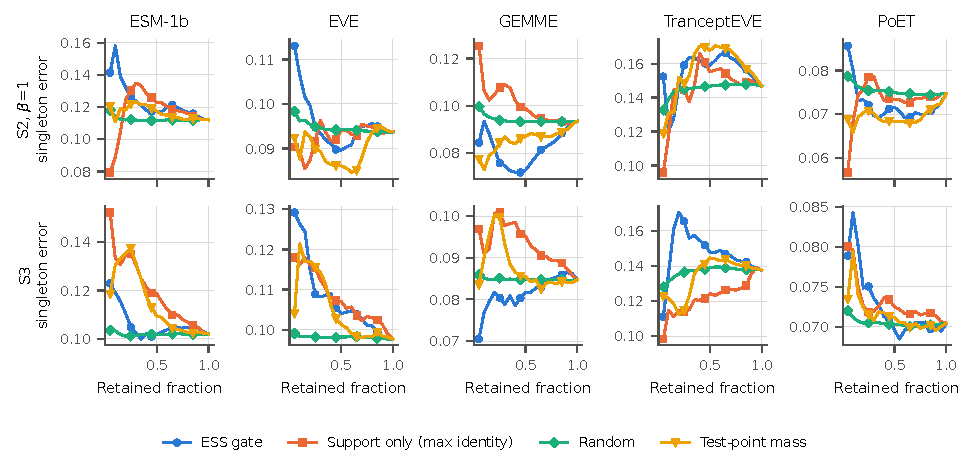
\includegraphics[width=\textwidth]{../figures/fig4_risk_coverage.pdf}
\caption{Risk-coverage of abstention rules applied to ProtCOVER-W's class-conditional sets ($\alpha=0.1$, mean over seeds): error of retained singleton sets as whole families are abstained in order of the score. Random abstention is averaged over 100 random family orders. The gate's decision depends only on label-free quantities, so it abstains on the same families whichever variant of (ii) it wraps.}
\label{fig:risk}
\end{figure}

Tables~\ref{tab:pairedpath}--\ref{tab:effsingerr} give paired differences between ProtCOVER and HCP, GWCP and ProtCOVER-W (class-conditional versions, $\alpha=0.1$, mean over seeds) with 95\% paired family-bootstrap intervals, which are conditional on the splits. Singleton error is the fraction of single-label sets that exclude the true label.

\begin{table}[h]
\caption{Paired differences in pathogenic coverage $\Cov_1$: ProtCOVER minus each baseline.}
\label{tab:pairedpath}
\centering\footnotesize\setlength{\tabcolsep}{3.5pt}
\begin{tabular}{llccc}
\toprule
 & & \multicolumn{3}{c}{$\Cov_1$ (pathogenic)} \\
\cmidrule(lr){3-5}
Setting & Predictor & $-$ HCP & $-$ GWCP & $-$ ProtCOVER-W \\
\midrule
S1 & ESM-1b & +0.001 [$-$0.003, +0.005] & +0.002 [$-$0.002, +0.006] & +0.006 [+0.003, +0.011] \\
 & EVE & $-$0.001 [$-$0.004, +0.001] & +0.001 [$-$0.002, +0.003] & $-$0.001 [$-$0.004, +0.001] \\
 & GEMME & +0.003 [$-$0.001, +0.006] & +0.004 [+0.001, +0.007] & +0.005 [+0.002, +0.009] \\
 & TranceptEVE & +0.005 [+0.003, +0.008] & +0.006 [+0.003, +0.009] & +0.004 [+0.001, +0.007] \\
 & PoET & +0.002 [$-$0.001, +0.005] & +0.002 [$-$0.001, +0.005] & +0.004 [+0.001, +0.007] \\
\midrule
S2, $\beta=1$ & ESM-1b & +0.071 [+0.065, +0.078] & +0.010 [+0.004, +0.017] & $-$0.001 [$-$0.008, +0.005] \\
 & EVE & +0.031 [+0.027, +0.036] & +0.009 [+0.005, +0.013] & +0.002 [$-$0.002, +0.007] \\
 & GEMME & +0.023 [+0.020, +0.027] & +0.012 [+0.008, +0.016] & +0.001 [$-$0.002, +0.005] \\
 & TranceptEVE & +0.015 [+0.012, +0.019] & +0.005 [+0.002, +0.008] & +0.002 [$-$0.000, +0.005] \\
 & PoET & $-$0.008 [$-$0.011, $-$0.006] & +0.008 [+0.005, +0.010] & +0.003 [+0.000, +0.005] \\
\midrule
S2, $\beta=2$ & ESM-1b & +0.131 [+0.124, +0.139] & +0.042 [+0.035, +0.049] & +0.027 [+0.021, +0.034] \\
 & EVE & +0.069 [+0.064, +0.075] & +0.047 [+0.042, +0.053] & +0.028 [+0.024, +0.032] \\
 & GEMME & +0.052 [+0.047, +0.057] & +0.034 [+0.029, +0.039] & +0.025 [+0.020, +0.029] \\
 & TranceptEVE & +0.052 [+0.048, +0.056] & +0.043 [+0.039, +0.048] & +0.024 [+0.021, +0.028] \\
 & PoET & $-$0.000 [$-$0.003, +0.003] & +0.025 [+0.021, +0.029] & +0.010 [+0.007, +0.013] \\
\midrule
S3 & ESM-1b & +0.014 [+0.011, +0.017] & +0.001 [$-$0.002, +0.004] & $-$0.004 [$-$0.006, $-$0.001] \\
 & EVE & $-$0.002 [$-$0.004, +0.000] & +0.004 [+0.002, +0.006] & +0.000 [$-$0.001, +0.002] \\
 & GEMME & +0.010 [+0.007, +0.012] & +0.005 [+0.002, +0.007] & +0.000 [$-$0.002, +0.002] \\
 & TranceptEVE & $-$0.012 [$-$0.014, $-$0.009] & $-$0.001 [$-$0.003, +0.002] & +0.002 [+0.000, +0.004] \\
 & PoET & $-$0.021 [$-$0.024, $-$0.018] & +0.009 [+0.007, +0.012] & +0.009 [+0.007, +0.012] \\
\midrule
S4 & ESM-1b & +0.021 [+0.018, +0.025] & +0.016 [+0.013, +0.020] & +0.026 [+0.022, +0.031] \\
 & EVE & +0.008 [+0.006, +0.011] & +0.015 [+0.012, +0.019] & +0.018 [+0.015, +0.022] \\
 & GEMME & +0.012 [+0.009, +0.014] & +0.015 [+0.012, +0.018] & +0.012 [+0.009, +0.014] \\
 & TranceptEVE & +0.004 [+0.002, +0.006] & +0.012 [+0.009, +0.014] & +0.023 [+0.020, +0.026] \\
 & PoET & +0.004 [+0.002, +0.007] & +0.016 [+0.013, +0.018] & +0.016 [+0.013, +0.019] \\
\bottomrule
\end{tabular}

\end{table}

\begin{table}[h]
\caption{Paired differences in benign coverage $\Cov_0$: ProtCOVER minus each baseline.}
\label{tab:pairedbenign}
\centering\footnotesize\setlength{\tabcolsep}{3.5pt}
\begin{tabular}{llccc}
\toprule
 & & \multicolumn{3}{c}{$\Cov_0$ (benign)} \\
\cmidrule(lr){3-5}
Setting & Predictor & $-$ HCP & $-$ GWCP & $-$ ProtCOVER-W \\
\midrule
S1 & ESM-1b & +0.002 [$-$0.000, +0.004] & +0.004 [+0.002, +0.006] & +0.001 [$-$0.001, +0.003] \\
 & EVE & +0.003 [+0.002, +0.005] & +0.005 [+0.004, +0.007] & +0.003 [+0.001, +0.004] \\
 & GEMME & +0.001 [$-$0.000, +0.003] & +0.003 [+0.001, +0.004] & +0.001 [$-$0.000, +0.002] \\
 & TranceptEVE & +0.004 [+0.002, +0.007] & +0.005 [+0.003, +0.008] & +0.003 [+0.001, +0.006] \\
 & PoET & +0.004 [+0.001, +0.007] & +0.006 [+0.004, +0.009] & +0.001 [$-$0.002, +0.004] \\
\midrule
S2, $\beta=1$ & ESM-1b & $-$0.016 [$-$0.019, $-$0.015] & +0.006 [+0.004, +0.009] & +0.006 [+0.004, +0.008] \\
 & EVE & $-$0.001 [$-$0.003, $-$0.000] & +0.006 [+0.005, +0.008] & +0.005 [+0.004, +0.007] \\
 & GEMME & +0.002 [+0.001, +0.004] & +0.008 [+0.006, +0.010] & +0.004 [+0.002, +0.005] \\
 & TranceptEVE & +0.012 [+0.010, +0.014] & +0.011 [+0.010, +0.013] & +0.007 [+0.006, +0.009] \\
 & PoET & +0.033 [+0.029, +0.036] & +0.010 [+0.007, +0.013] & +0.002 [$-$0.001, +0.006] \\
\midrule
S2, $\beta=2$ & ESM-1b & $-$0.020 [$-$0.022, $-$0.018] & +0.014 [+0.012, +0.016] & +0.004 [+0.001, +0.006] \\
 & EVE & +0.011 [+0.009, +0.013] & +0.021 [+0.019, +0.023] & +0.012 [+0.010, +0.014] \\
 & GEMME & +0.011 [+0.009, +0.013] & +0.028 [+0.026, +0.031] & +0.010 [+0.008, +0.012] \\
 & TranceptEVE & +0.030 [+0.027, +0.034] & +0.032 [+0.029, +0.036] & +0.022 [+0.019, +0.025] \\
 & PoET & +0.073 [+0.069, +0.078] & +0.053 [+0.049, +0.058] & +0.035 [+0.031, +0.039] \\
\midrule
S3 & ESM-1b & +0.002 [+0.000, +0.003] & +0.005 [+0.004, +0.006] & +0.002 [+0.001, +0.003] \\
 & EVE & +0.004 [+0.003, +0.005] & +0.004 [+0.003, +0.005] & +0.001 [+0.000, +0.002] \\
 & GEMME & +0.004 [+0.003, +0.005] & +0.009 [+0.007, +0.010] & +0.001 [+0.000, +0.002] \\
 & TranceptEVE & +0.025 [+0.023, +0.028] & +0.004 [+0.002, +0.007] & $-$0.004 [$-$0.005, $-$0.002] \\
 & PoET & +0.026 [+0.023, +0.029] & +0.004 [+0.002, +0.006] & $-$0.005 [$-$0.007, $-$0.003] \\
\midrule
S4 & ESM-1b & +0.006 [+0.004, +0.008] & +0.003 [+0.001, +0.006] & $-$0.000 [$-$0.002, +0.002] \\
 & EVE & +0.003 [+0.001, +0.004] & +0.001 [$-$0.001, +0.002] & $-$0.010 [$-$0.012, $-$0.008] \\
 & GEMME & +0.008 [+0.006, +0.009] & +0.010 [+0.008, +0.012] & +0.014 [+0.012, +0.017] \\
 & TranceptEVE & +0.016 [+0.014, +0.019] & +0.009 [+0.006, +0.011] & $-$0.010 [$-$0.012, $-$0.007] \\
 & PoET & +0.020 [+0.018, +0.023] & +0.014 [+0.011, +0.017] & $-$0.003 [$-$0.005, +0.000] \\
\bottomrule
\end{tabular}

\end{table}

\begin{table}[h]
\caption{Paired differences in mean set size (variant-weighted): ProtCOVER minus each baseline.}
\label{tab:effsize}
\centering\footnotesize\setlength{\tabcolsep}{3.5pt}
\begin{tabular}{llccc}
\toprule
 & & \multicolumn{3}{c}{Mean set size} \\
\cmidrule(lr){3-5}
Setting & Predictor & $-$ HCP & $-$ GWCP & $-$ ProtCOVER-W \\
\midrule
S1 & ESM-1b & $-$0.013 [$-$0.019, $-$0.006] & $-$0.009 [$-$0.015, $-$0.002] & $-$0.003 [$-$0.008, +0.004] \\
 & EVE & +0.010 [+0.006, +0.015] & +0.016 [+0.012, +0.021] & +0.006 [+0.003, +0.010] \\
 & GEMME & $-$0.004 [$-$0.008, $-$0.000] & $-$0.001 [$-$0.005, +0.003] & $-$0.001 [$-$0.005, +0.003] \\
 & TranceptEVE & +0.010 [$-$0.000, +0.019] & +0.013 [+0.003, +0.022] & +0.003 [$-$0.007, +0.012] \\
 & PoET & +0.009 [+0.002, +0.015] & +0.013 [+0.006, +0.019] & +0.009 [+0.002, +0.016] \\
\midrule
S2, $\beta=1$ & ESM-1b & +0.079 [+0.069, +0.091] & $-$0.020 [$-$0.031, $-$0.010] & $-$0.051 [$-$0.061, $-$0.040] \\
 & EVE & +0.041 [+0.035, +0.047] & +0.031 [+0.025, +0.037] & +0.021 [+0.016, +0.027] \\
 & GEMME & +0.047 [+0.041, +0.053] & +0.030 [+0.025, +0.037] & $-$0.003 [$-$0.008, +0.002] \\
 & TranceptEVE & +0.052 [+0.046, +0.059] & +0.034 [+0.027, +0.042] & +0.022 [+0.016, +0.029] \\
 & PoET & +0.020 [+0.014, +0.026] & +0.026 [+0.020, +0.033] & +0.000 [$-$0.005, +0.007] \\
\midrule
S2, $\beta=2$ & ESM-1b & +0.188 [+0.173, +0.204] & +0.055 [+0.042, +0.069] & +0.012 [+0.001, +0.024] \\
 & EVE & +0.170 [+0.158, +0.184] & +0.159 [+0.148, +0.173] & +0.114 [+0.105, +0.126] \\
 & GEMME & +0.150 [+0.138, +0.163] & +0.123 [+0.112, +0.135] & +0.080 [+0.073, +0.090] \\
 & TranceptEVE & +0.220 [+0.206, +0.237] & +0.206 [+0.192, +0.223] & +0.154 [+0.142, +0.168] \\
 & PoET & +0.149 [+0.137, +0.163] & +0.174 [+0.161, +0.189] & +0.117 [+0.106, +0.129] \\
\midrule
S3 & ESM-1b & +0.031 [+0.027, +0.037] & $-$0.001 [$-$0.005, +0.005] & $-$0.015 [$-$0.020, $-$0.010] \\
 & EVE & +0.012 [+0.010, +0.013] & +0.018 [+0.016, +0.020] & +0.006 [+0.005, +0.007] \\
 & GEMME & +0.029 [+0.026, +0.032] & +0.024 [+0.020, +0.027] & $-$0.001 [$-$0.004, +0.002] \\
 & TranceptEVE & +0.031 [+0.027, +0.035] & +0.007 [+0.003, +0.011] & $-$0.006 [$-$0.009, $-$0.003] \\
 & PoET & $-$0.005 [$-$0.009, $-$0.002] & +0.027 [+0.025, +0.030] & +0.010 [+0.007, +0.013] \\
\midrule
S4 & ESM-1b & +0.040 [+0.033, +0.047] & +0.035 [+0.027, +0.042] & +0.047 [+0.039, +0.055] \\
 & EVE & +0.037 [+0.029, +0.047] & +0.042 [+0.034, +0.051] & +0.005 [$-$0.001, +0.012] \\
 & GEMME & +0.052 [+0.043, +0.064] & +0.063 [+0.053, +0.074] & +0.048 [+0.039, +0.058] \\
 & TranceptEVE & +0.043 [+0.036, +0.050] & +0.044 [+0.036, +0.052] & +0.022 [+0.013, +0.031] \\
 & PoET & +0.041 [+0.034, +0.048] & +0.058 [+0.052, +0.065] & +0.028 [+0.023, +0.035] \\
\bottomrule
\end{tabular}

\end{table}

\begin{table}[h]
\caption{Paired differences in singleton error: ProtCOVER minus each baseline.}
\label{tab:effsingerr}
\centering\footnotesize\setlength{\tabcolsep}{3.5pt}
\begin{tabular}{llccc}
\toprule
 & & \multicolumn{3}{c}{Singleton error} \\
\cmidrule(lr){3-5}
Setting & Predictor & $-$ HCP & $-$ GWCP & $-$ ProtCOVER-W \\
\midrule
S1 & ESM-1b & $-$0.002 [$-$0.005, +0.001] & $-$0.003 [$-$0.006, $-$0.001] & $-$0.001 [$-$0.003, +0.002] \\
 & EVE & +0.002 [+0.001, +0.005] & +0.001 [$-$0.001, +0.003] & +0.003 [+0.001, +0.005] \\
 & GEMME & +0.000 [$-$0.002, +0.002] & $-$0.001 [$-$0.003, +0.001] & +0.001 [$-$0.001, +0.002] \\
 & TranceptEVE & +0.001 [$-$0.009, +0.012] & +0.000 [$-$0.009, +0.011] & +0.002 [$-$0.008, +0.013] \\
 & PoET & +0.008 [+0.005, +0.011] & +0.007 [+0.004, +0.010] & +0.008 [+0.006, +0.011] \\
\midrule
S2, $\beta=1$ & ESM-1b & +0.007 [+0.004, +0.010] & $-$0.010 [$-$0.014, $-$0.007] & $-$0.011 [$-$0.015, $-$0.007] \\
 & EVE & $-$0.000 [$-$0.002, +0.001] & $-$0.001 [$-$0.002, +0.001] & +0.001 [$-$0.001, +0.002] \\
 & GEMME & +0.002 [+0.001, +0.004] & $-$0.002 [$-$0.003, $-$0.001] & $-$0.000 [$-$0.002, +0.001] \\
 & TranceptEVE & +0.001 [$-$0.002, +0.004] & +0.008 [+0.004, +0.012] & +0.010 [+0.006, +0.014] \\
 & PoET & $-$0.013 [$-$0.015, $-$0.011] & $-$0.004 [$-$0.006, $-$0.002] & +0.000 [$-$0.002, +0.002] \\
\midrule
S2, $\beta=2$ & ESM-1b & +0.010 [+0.006, +0.015] & $-$0.014 [$-$0.018, $-$0.010] & $-$0.005 [$-$0.008, $-$0.001] \\
 & EVE & $-$0.004 [$-$0.006, $-$0.001] & $-$0.007 [$-$0.009, $-$0.004] & +0.001 [$-$0.001, +0.004] \\
 & GEMME & +0.002 [$-$0.001, +0.005] & $-$0.014 [$-$0.017, $-$0.010] & +0.000 [$-$0.003, +0.003] \\
 & TranceptEVE & +0.004 [$-$0.003, +0.010] & +0.008 [+0.000, +0.015] & +0.018 [+0.011, +0.024] \\
 & PoET & $-$0.026 [$-$0.029, $-$0.022] & $-$0.018 [$-$0.021, $-$0.015] & $-$0.007 [$-$0.010, $-$0.005] \\
\midrule
S3 & ESM-1b & $-$0.002 [$-$0.003, $-$0.001] & $-$0.005 [$-$0.007, $-$0.004] & $-$0.004 [$-$0.005, $-$0.002] \\
 & EVE & $-$0.003 [$-$0.004, $-$0.002] & $-$0.004 [$-$0.005, $-$0.003] & $-$0.001 [$-$0.002, $-$0.000] \\
 & GEMME & $-$0.002 [$-$0.004, $-$0.001] & $-$0.004 [$-$0.006, $-$0.003] & $-$0.001 [$-$0.003, +0.000] \\
 & TranceptEVE & +0.004 [+0.001, +0.008] & $-$0.001 [$-$0.003, +0.002] & $-$0.001 [$-$0.003, +0.000] \\
 & PoET & $-$0.004 [$-$0.006, $-$0.003] & $-$0.001 [$-$0.002, +0.001] & +0.003 [+0.001, +0.004] \\
\midrule
S4 & ESM-1b & $-$0.002 [$-$0.004, +0.000] & $-$0.001 [$-$0.003, +0.001] & $-$0.001 [$-$0.003, +0.002] \\
 & EVE & +0.001 [$-$0.001, +0.002] & $-$0.001 [$-$0.002, +0.000] & +0.001 [$-$0.000, +0.003] \\
 & GEMME & +0.002 [+0.001, +0.003] & $-$0.000 [$-$0.002, +0.001] & $-$0.002 [$-$0.004, $-$0.000] \\
 & TranceptEVE & $-$0.004 [$-$0.011, +0.001] & $-$0.013 [$-$0.021, $-$0.006] & $-$0.024 [$-$0.032, $-$0.016] \\
 & PoET & $-$0.005 [$-$0.006, $-$0.003] & $-$0.004 [$-$0.006, $-$0.003] & +0.001 [$-$0.001, +0.003] \\
\bottomrule
\end{tabular}

\end{table}

Tables~\ref{tab:full10}--\ref{tab:full20} report every method, marginal (cc $=$ no) and class-conditional (cc $=$ yes), averaged over the five predictors: family-weighted coverage $\Cov$, variant-weighted coverage, $\Cov_1$, $\Cov_0$, mean set size, singleton rate, the fraction of families with at least ten variants whose coverage is below $1-\alpha-0.05$, and the fraction of test families on which the method abstained. Per-predictor values with bootstrap intervals, and the summaries of every sensitivity, stress and external run, are in \path{results/} of the code repository.

{\footnotesize\setlength{\tabcolsep}{2.5pt}
\begin{tabular}{llccccccccc}
\toprule
Setting & Method & cc & $\Cov$ & var.-w. & $\Cov_1$ & $\Cov_0$ & size & single. & under-cov. & abst. \\
\midrule
S1 (exchangeable) & Split (B1/B2) & no & 0.882 & 0.899 & 0.798 & 0.884 & 1.143 & 0.857 & 0.237 & 0.000 \\
 & Split (B1/B2) & yes & 0.881 & 0.898 & 0.800 & 0.881 & 1.142 & 0.858 & 0.240 & 0.000 \\
 & HCP (B3) & no & 0.901 & 0.918 & 0.827 & 0.903 & 1.204 & 0.796 & 0.180 & 0.000 \\
 & HCP (B3) & yes & 0.922 & 0.929 & 0.901 & 0.901 & 1.304 & 0.696 & 0.134 & 0.000 \\
 & Subsample once (B3) & no & 0.900 & 0.918 & 0.828 & 0.902 & 1.204 & 0.796 & 0.180 & 0.000 \\
 & Subsample once (B3) & yes & 0.922 & 0.929 & 0.901 & 0.900 & 1.305 & 0.695 & 0.136 & 0.000 \\
 & Repeated subsample (B3) & no & 0.901 & 0.918 & 0.826 & 0.903 & 1.205 & 0.795 & 0.180 & 0.000 \\
 & Repeated subsample (B3) & yes & 0.923 & 0.929 & 0.901 & 0.901 & 1.305 & 0.695 & 0.134 & 0.000 \\
 & GWCP (B4) & no & 0.899 & 0.917 & 0.824 & 0.901 & 1.199 & 0.801 & 0.185 & 0.000 \\
 & GWCP (B4) & yes & 0.921 & 0.928 & 0.900 & 0.899 & 1.300 & 0.700 & 0.136 & 0.000 \\
 & ProtCOVER (i)+(ii) & no & 0.900 & 0.918 & 0.826 & 0.903 & 1.204 & 0.796 & 0.181 & 0.000 \\
 & ProtCOVER (i)+(ii) & yes & 0.923 & 0.930 & 0.899 & 0.902 & 1.303 & 0.697 & 0.133 & 0.000 \\
 & ProtCOVER (i)+(iii) & no & 0.901 & 0.918 & 0.827 & 0.903 & 1.204 & 0.796 & 0.180 & 0.000 \\
 & ProtCOVER (i)+(iii) & yes & 0.923 & 0.929 & 0.901 & 0.901 & 1.304 & 0.696 & 0.134 & 0.000 \\
 & ProtCOVER full & no & 0.901 & 0.918 & 0.826 & 0.903 & 1.204 & 0.796 & 0.180 & 0.000 \\
 & ProtCOVER full & yes & 0.923 & 0.930 & 0.899 & 0.903 & 1.304 & 0.696 & 0.133 & 0.000 \\
 & Support-only abst. (B5) & no & 0.901 & 0.918 & 0.826 & 0.903 & 1.204 & 0.796 & 0.181 & 0.000 \\
 & Support-only abst. (B5) & yes & 0.923 & 0.930 & 0.899 & 0.902 & 1.304 & 0.696 & 0.133 & 0.000 \\
 & Random abst. (B5) & no & 0.901 & 0.918 & 0.826 & 0.903 & 1.204 & 0.796 & 0.180 & 0.000 \\
 & Random abst. (B5) & yes & 0.923 & 0.930 & 0.899 & 0.902 & 1.304 & 0.696 & 0.133 & 0.000 \\
\midrule
S2, $\beta=1$ & Split (B1/B2) & no & 0.875 & 0.893 & 0.772 & 0.883 & 1.137 & 0.863 & 0.252 & 0.000 \\
 & Split (B1/B2) & yes & 0.873 & 0.891 & 0.758 & 0.889 & 1.137 & 0.863 & 0.255 & 0.000 \\
 & HCP (B3) & no & 0.893 & 0.912 & 0.800 & 0.901 & 1.195 & 0.805 & 0.200 & 0.000 \\
 & HCP (B3) & yes & 0.917 & 0.925 & 0.875 & 0.904 & 1.291 & 0.709 & 0.147 & 0.000 \\
 & Subsample once (B3) & no & 0.893 & 0.912 & 0.800 & 0.902 & 1.195 & 0.805 & 0.200 & 0.000 \\
 & Subsample once (B3) & yes & 0.918 & 0.926 & 0.877 & 0.904 & 1.294 & 0.706 & 0.146 & 0.000 \\
 & Repeated subsample (B3) & no & 0.893 & 0.912 & 0.800 & 0.901 & 1.195 & 0.805 & 0.200 & 0.000 \\
 & Repeated subsample (B3) & yes & 0.917 & 0.925 & 0.875 & 0.904 & 1.290 & 0.710 & 0.147 & 0.000 \\
 & GWCP (B4) & no & 0.896 & 0.914 & 0.805 & 0.903 & 1.202 & 0.798 & 0.195 & 0.000 \\
 & GWCP (B4) & yes & 0.921 & 0.928 & 0.893 & 0.902 & 1.318 & 0.682 & 0.140 & 0.000 \\
 & ProtCOVER (i)+(ii) & no & 0.903 & 0.921 & 0.818 & 0.909 & 1.227 & 0.773 & 0.176 & 0.000 \\
 & ProtCOVER (i)+(ii) & yes & 0.925 & 0.931 & 0.900 & 0.905 & 1.340 & 0.660 & 0.130 & 0.000 \\
 & ProtCOVER (i)+(iii) & no & 0.893 & 0.912 & 0.800 & 0.901 & 1.195 & 0.805 & 0.200 & 0.000 \\
 & ProtCOVER (i)+(iii) & yes & 0.917 & 0.925 & 0.875 & 0.904 & 1.291 & 0.709 & 0.147 & 0.000 \\
 & ProtCOVER full & no & 0.903 & 0.921 & 0.818 & 0.909 & 1.227 & 0.773 & 0.176 & 0.000 \\
 & ProtCOVER full & yes & 0.925 & 0.931 & 0.900 & 0.905 & 1.340 & 0.660 & 0.129 & 0.000 \\
 & Support-only abst. (B5) & no & 0.903 & 0.921 & 0.818 & 0.909 & 1.227 & 0.773 & 0.176 & 0.000 \\
 & Support-only abst. (B5) & yes & 0.925 & 0.931 & 0.900 & 0.905 & 1.341 & 0.659 & 0.130 & 0.000 \\
 & Random abst. (B5) & no & 0.903 & 0.921 & 0.818 & 0.909 & 1.227 & 0.773 & 0.176 & 0.000 \\
 & Random abst. (B5) & yes & 0.925 & 0.931 & 0.900 & 0.905 & 1.341 & 0.659 & 0.130 & 0.000 \\
\midrule
S2, $\beta=2$ & Split (B1/B2) & no & 0.874 & 0.892 & 0.764 & 0.883 & 1.136 & 0.864 & 0.255 & 0.000 \\
 & Split (B1/B2) & yes & 0.871 & 0.890 & 0.746 & 0.889 & 1.136 & 0.864 & 0.259 & 0.000 \\
 & HCP (B3) & no & 0.892 & 0.911 & 0.793 & 0.900 & 1.192 & 0.808 & 0.204 & 0.000 \\
 & HCP (B3) & yes & 0.914 & 0.923 & 0.864 & 0.903 & 1.283 & 0.717 & 0.156 & 0.000 \\
 & Subsample once (B3) & no & 0.889 & 0.909 & 0.792 & 0.896 & 1.187 & 0.813 & 0.211 & 0.000 \\
 & Subsample once (B3) & yes & 0.912 & 0.922 & 0.863 & 0.901 & 1.279 & 0.721 & 0.159 & 0.000 \\
 & Repeated subsample (B3) & no & 0.891 & 0.911 & 0.792 & 0.900 & 1.192 & 0.808 & 0.204 & 0.000 \\
 & Repeated subsample (B3) & yes & 0.914 & 0.923 & 0.864 & 0.903 & 1.283 & 0.717 & 0.156 & 0.000 \\
 & GWCP (B4) & no & 0.896 & 0.915 & 0.801 & 0.904 & 1.212 & 0.788 & 0.196 & 0.000 \\
 & GWCP (B4) & yes & 0.915 & 0.923 & 0.887 & 0.894 & 1.315 & 0.685 & 0.159 & 0.000 \\
 & ProtCOVER (i)+(ii) & no & 0.909 & 0.927 & 0.826 & 0.914 & 1.260 & 0.740 & 0.161 & 0.000 \\
 & ProtCOVER (i)+(ii) & yes & 0.927 & 0.935 & 0.902 & 0.907 & 1.363 & 0.637 & 0.127 & 0.000 \\
 & ProtCOVER (i)+(iii) & no & 0.892 & 0.911 & 0.793 & 0.900 & 1.192 & 0.808 & 0.204 & 0.000 \\
 & ProtCOVER (i)+(iii) & yes & 0.914 & 0.923 & 0.864 & 0.903 & 1.283 & 0.717 & 0.156 & 0.000 \\
 & ProtCOVER full & no & 0.909 & 0.927 & 0.827 & 0.914 & 1.264 & 0.736 & 0.161 & 0.004 \\
 & ProtCOVER full & yes & 0.928 & 0.936 & 0.904 & 0.908 & 1.372 & 0.628 & 0.125 & 0.022 \\
 & Support-only abst. (B5) & no & 0.909 & 0.927 & 0.827 & 0.914 & 1.263 & 0.737 & 0.160 & 0.004 \\
 & Support-only abst. (B5) & yes & 0.928 & 0.936 & 0.904 & 0.909 & 1.375 & 0.625 & 0.125 & 0.022 \\
 & Random abst. (B5) & no & 0.909 & 0.928 & 0.827 & 0.915 & 1.264 & 0.736 & 0.160 & 0.004 \\
 & Random abst. (B5) & yes & 0.928 & 0.936 & 0.904 & 0.909 & 1.375 & 0.625 & 0.125 & 0.022 \\
\midrule
S3 (orphan families) & Split (B1/B2) & no & 0.875 & 0.891 & 0.789 & 0.878 & 1.137 & 0.863 & 0.254 & 0.000 \\
 & Split (B1/B2) & yes & 0.874 & 0.890 & 0.787 & 0.878 & 1.135 & 0.865 & 0.251 & 0.000 \\
 & HCP (B3) & no & 0.897 & 0.913 & 0.821 & 0.899 & 1.204 & 0.796 & 0.193 & 0.000 \\
 & HCP (B3) & yes & 0.922 & 0.931 & 0.904 & 0.896 & 1.308 & 0.692 & 0.129 & 0.000 \\
 & Subsample once (B3) & no & 0.896 & 0.912 & 0.820 & 0.898 & 1.204 & 0.796 & 0.195 & 0.000 \\
 & Subsample once (B3) & yes & 0.922 & 0.931 & 0.904 & 0.896 & 1.309 & 0.691 & 0.128 & 0.000 \\
 & Repeated subsample (B3) & no & 0.896 & 0.912 & 0.821 & 0.899 & 1.203 & 0.797 & 0.194 & 0.000 \\
 & Repeated subsample (B3) & yes & 0.922 & 0.931 & 0.904 & 0.896 & 1.308 & 0.692 & 0.129 & 0.000 \\
 & GWCP (B4) & no & 0.901 & 0.917 & 0.827 & 0.903 & 1.220 & 0.780 & 0.182 & 0.000 \\
 & GWCP (B4) & yes & 0.924 & 0.931 & 0.898 & 0.903 & 1.312 & 0.688 & 0.128 & 0.000 \\
 & ProtCOVER (i)+(ii) & no & 0.905 & 0.922 & 0.834 & 0.908 & 1.238 & 0.762 & 0.170 & 0.000 \\
 & ProtCOVER (i)+(ii) & yes & 0.928 & 0.934 & 0.900 & 0.910 & 1.329 & 0.671 & 0.120 & 0.000 \\
 & ProtCOVER (i)+(iii) & no & 0.897 & 0.913 & 0.821 & 0.899 & 1.204 & 0.796 & 0.193 & 0.000 \\
 & ProtCOVER (i)+(iii) & yes & 0.922 & 0.931 & 0.904 & 0.897 & 1.309 & 0.691 & 0.129 & 0.003 \\
 & ProtCOVER full & no & 0.905 & 0.922 & 0.834 & 0.908 & 1.238 & 0.762 & 0.170 & 0.000 \\
 & ProtCOVER full & yes & 0.928 & 0.934 & 0.901 & 0.910 & 1.331 & 0.669 & 0.120 & 0.004 \\
 & Support-only abst. (B5) & no & 0.905 & 0.922 & 0.834 & 0.908 & 1.238 & 0.762 & 0.170 & 0.000 \\
 & Support-only abst. (B5) & yes & 0.928 & 0.934 & 0.901 & 0.910 & 1.331 & 0.669 & 0.120 & 0.004 \\
 & Random abst. (B5) & no & 0.905 & 0.922 & 0.834 & 0.908 & 1.238 & 0.762 & 0.170 & 0.000 \\
 & Random abst. (B5) & yes & 0.928 & 0.934 & 0.901 & 0.910 & 1.331 & 0.669 & 0.120 & 0.004 \\
\midrule
S4 (held-out regions) & Split (B1/B2) & no & 0.878 & 0.895 & 0.801 & 0.882 & 1.145 & 0.855 & 0.245 & 0.000 \\
 & Split (B1/B2) & yes & 0.876 & 0.895 & 0.802 & 0.877 & 1.141 & 0.859 & 0.248 & 0.000 \\
 & HCP (B3) & no & 0.897 & 0.915 & 0.830 & 0.900 & 1.205 & 0.795 & 0.188 & 0.000 \\
 & HCP (B3) & yes & 0.920 & 0.928 & 0.904 & 0.896 & 1.300 & 0.700 & 0.137 & 0.000 \\
 & Subsample once (B3) & no & 0.899 & 0.916 & 0.835 & 0.900 & 1.212 & 0.788 & 0.186 & 0.000 \\
 & Subsample once (B3) & yes & 0.920 & 0.928 & 0.904 & 0.896 & 1.301 & 0.699 & 0.138 & 0.000 \\
 & Repeated subsample (B3) & no & 0.897 & 0.914 & 0.829 & 0.900 & 1.205 & 0.795 & 0.189 & 0.000 \\
 & Repeated subsample (B3) & yes & 0.920 & 0.928 & 0.904 & 0.896 & 1.300 & 0.700 & 0.137 & 0.000 \\
 & GWCP (B4) & no & 0.897 & 0.915 & 0.830 & 0.901 & 1.207 & 0.793 & 0.188 & 0.000 \\
 & GWCP (B4) & yes & 0.920 & 0.926 & 0.899 & 0.899 & 1.294 & 0.706 & 0.141 & 0.000 \\
 & ProtCOVER (i)+(ii) & no & 0.903 & 0.919 & 0.836 & 0.907 & 1.232 & 0.768 & 0.177 & 0.000 \\
 & ProtCOVER (i)+(ii) & yes & 0.923 & 0.926 & 0.895 & 0.908 & 1.312 & 0.688 & 0.138 & 0.000 \\
 & ProtCOVER (i)+(iii) & no & 0.897 & 0.915 & 0.830 & 0.901 & 1.207 & 0.793 & 0.188 & 0.001 \\
 & ProtCOVER (i)+(iii) & yes & 0.920 & 0.928 & 0.904 & 0.896 & 1.304 & 0.696 & 0.137 & 0.003 \\
 & ProtCOVER full & no & 0.903 & 0.919 & 0.837 & 0.907 & 1.233 & 0.767 & 0.177 & 0.001 \\
 & ProtCOVER full & yes & 0.923 & 0.926 & 0.895 & 0.909 & 1.316 & 0.684 & 0.137 & 0.005 \\
 & Support-only abst. (B5) & no & 0.903 & 0.919 & 0.837 & 0.907 & 1.232 & 0.768 & 0.177 & 0.001 \\
 & Support-only abst. (B5) & yes & 0.923 & 0.926 & 0.896 & 0.908 & 1.315 & 0.685 & 0.137 & 0.005 \\
 & Random abst. (B5) & no & 0.903 & 0.919 & 0.837 & 0.907 & 1.232 & 0.768 & 0.177 & 0.001 \\
 & Random abst. (B5) & yes & 0.923 & 0.926 & 0.896 & 0.908 & 1.315 & 0.685 & 0.137 & 0.005 \\
\bottomrule
\end{tabular}
}

{\footnotesize\setlength{\tabcolsep}{2.5pt}
\begin{tabular}{llccccccccc}
\toprule
Setting & Method & cc & $\Cov$ & var.-w. & $\Cov_1$ & $\Cov_0$ & size & single. & under-cov. & abst. \\
\midrule
S1 (exchangeable) & Split (B1/B2) & no & 0.933 & 0.949 & 0.876 & 0.934 & 1.336 & 0.664 & 0.152 & 0.000 \\
 & Split (B1/B2) & yes & 0.933 & 0.949 & 0.876 & 0.936 & 1.335 & 0.665 & 0.151 & 0.000 \\
 & HCP (B3) & no & 0.950 & 0.966 & 0.904 & 0.953 & 1.443 & 0.557 & 0.095 & 0.000 \\
 & HCP (B3) & yes & 0.963 & 0.968 & 0.952 & 0.950 & 1.517 & 0.483 & 0.075 & 0.000 \\
 & Subsample once (B3) & no & 0.950 & 0.965 & 0.902 & 0.952 & 1.441 & 0.559 & 0.098 & 0.000 \\
 & Subsample once (B3) & yes & 0.963 & 0.967 & 0.951 & 0.950 & 1.515 & 0.485 & 0.076 & 0.000 \\
 & Repeated subsample (B3) & no & 0.951 & 0.966 & 0.904 & 0.953 & 1.444 & 0.556 & 0.094 & 0.000 \\
 & Repeated subsample (B3) & yes & 0.963 & 0.968 & 0.952 & 0.950 & 1.517 & 0.483 & 0.076 & 0.000 \\
 & GWCP (B4) & no & 0.949 & 0.964 & 0.901 & 0.951 & 1.432 & 0.568 & 0.101 & 0.000 \\
 & GWCP (B4) & yes & 0.961 & 0.966 & 0.950 & 0.948 & 1.507 & 0.493 & 0.080 & 0.000 \\
 & ProtCOVER (i)+(ii) & no & 0.951 & 0.966 & 0.904 & 0.953 & 1.445 & 0.555 & 0.094 & 0.000 \\
 & ProtCOVER (i)+(ii) & yes & 0.964 & 0.969 & 0.951 & 0.952 & 1.523 & 0.477 & 0.073 & 0.000 \\
 & ProtCOVER (i)+(iii) & no & 0.950 & 0.966 & 0.904 & 0.953 & 1.443 & 0.557 & 0.095 & 0.000 \\
 & ProtCOVER (i)+(iii) & yes & 0.963 & 0.968 & 0.952 & 0.950 & 1.517 & 0.483 & 0.075 & 0.000 \\
 & ProtCOVER full & no & 0.951 & 0.966 & 0.904 & 0.953 & 1.445 & 0.555 & 0.094 & 0.000 \\
 & ProtCOVER full & yes & 0.964 & 0.969 & 0.951 & 0.952 & 1.523 & 0.477 & 0.073 & 0.000 \\
 & Support-only abst. (B5) & no & 0.951 & 0.966 & 0.904 & 0.953 & 1.445 & 0.555 & 0.094 & 0.000 \\
 & Support-only abst. (B5) & yes & 0.964 & 0.969 & 0.951 & 0.952 & 1.523 & 0.477 & 0.073 & 0.000 \\
 & Random abst. (B5) & no & 0.951 & 0.966 & 0.904 & 0.953 & 1.445 & 0.555 & 0.094 & 0.000 \\
 & Random abst. (B5) & yes & 0.964 & 0.969 & 0.951 & 0.952 & 1.523 & 0.477 & 0.073 & 0.000 \\
\midrule
S2, $\beta=1$ & Split (B1/B2) & no & 0.928 & 0.946 & 0.859 & 0.934 & 1.330 & 0.670 & 0.167 & 0.000 \\
 & Split (B1/B2) & yes & 0.927 & 0.944 & 0.843 & 0.940 & 1.325 & 0.675 & 0.167 & 0.000 \\
 & HCP (B3) & no & 0.946 & 0.962 & 0.889 & 0.950 & 1.431 & 0.569 & 0.108 & 0.000 \\
 & HCP (B3) & yes & 0.960 & 0.967 & 0.936 & 0.952 & 1.516 & 0.484 & 0.080 & 0.000 \\
 & Subsample once (B3) & no & 0.947 & 0.963 & 0.890 & 0.951 & 1.441 & 0.559 & 0.105 & 0.000 \\
 & Subsample once (B3) & yes & 0.958 & 0.966 & 0.935 & 0.949 & 1.510 & 0.490 & 0.084 & 0.000 \\
 & Repeated subsample (B3) & no & 0.946 & 0.962 & 0.889 & 0.950 & 1.432 & 0.568 & 0.109 & 0.000 \\
 & Repeated subsample (B3) & yes & 0.960 & 0.967 & 0.935 & 0.952 & 1.515 & 0.485 & 0.080 & 0.000 \\
 & GWCP (B4) & no & 0.947 & 0.964 & 0.892 & 0.951 & 1.447 & 0.553 & 0.104 & 0.000 \\
 & GWCP (B4) & yes & 0.961 & 0.966 & 0.944 & 0.950 & 1.527 & 0.473 & 0.081 & 0.000 \\
 & ProtCOVER (i)+(ii) & no & 0.954 & 0.969 & 0.905 & 0.957 & 1.489 & 0.511 & 0.086 & 0.000 \\
 & ProtCOVER (i)+(ii) & yes & 0.965 & 0.969 & 0.951 & 0.955 & 1.553 & 0.447 & 0.069 & 0.000 \\
 & ProtCOVER (i)+(iii) & no & 0.946 & 0.962 & 0.889 & 0.950 & 1.431 & 0.569 & 0.108 & 0.000 \\
 & ProtCOVER (i)+(iii) & yes & 0.960 & 0.967 & 0.936 & 0.952 & 1.516 & 0.484 & 0.080 & 0.000 \\
 & ProtCOVER full & no & 0.954 & 0.969 & 0.905 & 0.957 & 1.489 & 0.511 & 0.086 & 0.000 \\
 & ProtCOVER full & yes & 0.965 & 0.969 & 0.951 & 0.955 & 1.553 & 0.447 & 0.069 & 0.000 \\
 & Support-only abst. (B5) & no & 0.954 & 0.969 & 0.905 & 0.957 & 1.489 & 0.511 & 0.086 & 0.000 \\
 & Support-only abst. (B5) & yes & 0.965 & 0.969 & 0.951 & 0.955 & 1.554 & 0.446 & 0.069 & 0.000 \\
 & Random abst. (B5) & no & 0.954 & 0.969 & 0.905 & 0.957 & 1.489 & 0.511 & 0.086 & 0.000 \\
 & Random abst. (B5) & yes & 0.965 & 0.969 & 0.951 & 0.955 & 1.554 & 0.446 & 0.069 & 0.000 \\
\midrule
S2, $\beta=2$ & Split (B1/B2) & no & 0.927 & 0.945 & 0.852 & 0.933 & 1.329 & 0.671 & 0.170 & 0.000 \\
 & Split (B1/B2) & yes & 0.925 & 0.943 & 0.833 & 0.941 & 1.324 & 0.676 & 0.173 & 0.000 \\
 & HCP (B3) & no & 0.944 & 0.961 & 0.884 & 0.949 & 1.427 & 0.573 & 0.114 & 0.000 \\
 & HCP (B3) & yes & 0.957 & 0.966 & 0.929 & 0.950 & 1.512 & 0.488 & 0.087 & 0.000 \\
 & Subsample once (B3) & no & 0.943 & 0.959 & 0.878 & 0.949 & 1.416 & 0.584 & 0.119 & 0.000 \\
 & Subsample once (B3) & yes & 0.956 & 0.964 & 0.926 & 0.949 & 1.505 & 0.495 & 0.090 & 0.000 \\
 & Repeated subsample (B3) & no & 0.945 & 0.961 & 0.883 & 0.949 & 1.427 & 0.573 & 0.115 & 0.000 \\
 & Repeated subsample (B3) & yes & 0.957 & 0.966 & 0.929 & 0.949 & 1.511 & 0.489 & 0.087 & 0.000 \\
 & GWCP (B4) & no & 0.946 & 0.963 & 0.888 & 0.950 & 1.456 & 0.544 & 0.109 & 0.000 \\
 & GWCP (B4) & yes & 0.956 & 0.963 & 0.943 & 0.942 & 1.526 & 0.474 & 0.096 & 0.000 \\
 & ProtCOVER (i)+(ii) & no & 0.962 & 0.975 & 0.924 & 0.963 & 1.572 & 0.428 & 0.068 & 0.000 \\
 & ProtCOVER (i)+(ii) & yes & 0.969 & 0.974 & 0.962 & 0.958 & 1.612 & 0.388 & 0.064 & 0.000 \\
 & ProtCOVER (i)+(iii) & no & 0.944 & 0.961 & 0.884 & 0.949 & 1.427 & 0.573 & 0.114 & 0.000 \\
 & ProtCOVER (i)+(iii) & yes & 0.957 & 0.966 & 0.929 & 0.950 & 1.512 & 0.488 & 0.087 & 0.000 \\
 & ProtCOVER full & no & 0.962 & 0.975 & 0.924 & 0.963 & 1.572 & 0.428 & 0.068 & 0.000 \\
 & ProtCOVER full & yes & 0.969 & 0.974 & 0.962 & 0.958 & 1.613 & 0.387 & 0.064 & 0.014 \\
 & Support-only abst. (B5) & no & 0.962 & 0.975 & 0.924 & 0.963 & 1.572 & 0.428 & 0.068 & 0.000 \\
 & Support-only abst. (B5) & yes & 0.969 & 0.974 & 0.962 & 0.958 & 1.617 & 0.383 & 0.063 & 0.014 \\
 & Random abst. (B5) & no & 0.962 & 0.975 & 0.924 & 0.963 & 1.572 & 0.428 & 0.068 & 0.000 \\
 & Random abst. (B5) & yes & 0.969 & 0.974 & 0.962 & 0.958 & 1.616 & 0.384 & 0.063 & 0.014 \\
\midrule
S3 (orphan families) & Split (B1/B2) & no & 0.929 & 0.944 & 0.870 & 0.931 & 1.330 & 0.670 & 0.159 & 0.000 \\
 & Split (B1/B2) & yes & 0.930 & 0.944 & 0.865 & 0.936 & 1.330 & 0.670 & 0.156 & 0.000 \\
 & HCP (B3) & no & 0.949 & 0.963 & 0.903 & 0.951 & 1.448 & 0.552 & 0.096 & 0.000 \\
 & HCP (B3) & yes & 0.963 & 0.970 & 0.952 & 0.950 & 1.527 & 0.473 & 0.069 & 0.000 \\
 & Subsample once (B3) & no & 0.946 & 0.961 & 0.899 & 0.948 & 1.440 & 0.560 & 0.105 & 0.000 \\
 & Subsample once (B3) & yes & 0.962 & 0.970 & 0.952 & 0.948 & 1.525 & 0.475 & 0.070 & 0.000 \\
 & Repeated subsample (B3) & no & 0.949 & 0.963 & 0.903 & 0.951 & 1.447 & 0.553 & 0.097 & 0.000 \\
 & Repeated subsample (B3) & yes & 0.963 & 0.970 & 0.952 & 0.950 & 1.528 & 0.472 & 0.068 & 0.000 \\
 & GWCP (B4) & no & 0.951 & 0.965 & 0.905 & 0.954 & 1.467 & 0.533 & 0.091 & 0.000 \\
 & GWCP (B4) & yes & 0.964 & 0.969 & 0.951 & 0.953 & 1.527 & 0.473 & 0.069 & 0.000 \\
 & ProtCOVER (i)+(ii) & no & 0.956 & 0.969 & 0.912 & 0.959 & 1.499 & 0.501 & 0.078 & 0.000 \\
 & ProtCOVER (i)+(ii) & yes & 0.967 & 0.971 & 0.953 & 0.958 & 1.548 & 0.452 & 0.063 & 0.000 \\
 & ProtCOVER (i)+(iii) & no & 0.949 & 0.963 & 0.903 & 0.951 & 1.448 & 0.552 & 0.096 & 0.000 \\
 & ProtCOVER (i)+(iii) & yes & 0.963 & 0.970 & 0.952 & 0.950 & 1.527 & 0.473 & 0.069 & 0.000 \\
 & ProtCOVER full & no & 0.956 & 0.969 & 0.912 & 0.959 & 1.499 & 0.501 & 0.078 & 0.000 \\
 & ProtCOVER full & yes & 0.967 & 0.971 & 0.953 & 0.958 & 1.548 & 0.452 & 0.063 & 0.000 \\
 & Support-only abst. (B5) & no & 0.956 & 0.969 & 0.912 & 0.959 & 1.499 & 0.501 & 0.078 & 0.000 \\
 & Support-only abst. (B5) & yes & 0.967 & 0.971 & 0.953 & 0.958 & 1.548 & 0.452 & 0.063 & 0.000 \\
 & Random abst. (B5) & no & 0.956 & 0.969 & 0.912 & 0.959 & 1.499 & 0.501 & 0.078 & 0.000 \\
 & Random abst. (B5) & yes & 0.967 & 0.971 & 0.953 & 0.958 & 1.548 & 0.452 & 0.063 & 0.000 \\
\midrule
S4 (held-out regions) & Split (B1/B2) & no & 0.930 & 0.947 & 0.879 & 0.933 & 1.340 & 0.660 & 0.154 & 0.000 \\
 & Split (B1/B2) & yes & 0.931 & 0.947 & 0.878 & 0.932 & 1.337 & 0.663 & 0.155 & 0.000 \\
 & HCP (B3) & no & 0.949 & 0.964 & 0.907 & 0.951 & 1.447 & 0.553 & 0.097 & 0.000 \\
 & HCP (B3) & yes & 0.961 & 0.967 & 0.953 & 0.946 & 1.510 & 0.490 & 0.077 & 0.000 \\
 & Subsample once (B3) & no & 0.948 & 0.964 & 0.907 & 0.950 & 1.445 & 0.555 & 0.099 & 0.000 \\
 & Subsample once (B3) & yes & 0.960 & 0.966 & 0.952 & 0.946 & 1.506 & 0.494 & 0.077 & 0.000 \\
 & Repeated subsample (B3) & no & 0.949 & 0.964 & 0.908 & 0.951 & 1.448 & 0.552 & 0.096 & 0.000 \\
 & Repeated subsample (B3) & yes & 0.961 & 0.967 & 0.953 & 0.946 & 1.509 & 0.491 & 0.077 & 0.000 \\
 & GWCP (B4) & no & 0.948 & 0.963 & 0.906 & 0.950 & 1.442 & 0.558 & 0.101 & 0.000 \\
 & GWCP (B4) & yes & 0.960 & 0.965 & 0.950 & 0.947 & 1.503 & 0.497 & 0.080 & 0.000 \\
 & ProtCOVER (i)+(ii) & no & 0.953 & 0.967 & 0.912 & 0.956 & 1.488 & 0.512 & 0.089 & 0.000 \\
 & ProtCOVER (i)+(ii) & yes & 0.962 & 0.965 & 0.948 & 0.953 & 1.528 & 0.472 & 0.080 & 0.000 \\
 & ProtCOVER (i)+(iii) & no & 0.949 & 0.964 & 0.907 & 0.951 & 1.447 & 0.553 & 0.097 & 0.000 \\
 & ProtCOVER (i)+(iii) & yes & 0.961 & 0.967 & 0.954 & 0.947 & 1.515 & 0.485 & 0.076 & 0.007 \\
 & ProtCOVER full & no & 0.953 & 0.967 & 0.912 & 0.956 & 1.488 & 0.512 & 0.089 & 0.000 \\
 & ProtCOVER full & yes & 0.962 & 0.965 & 0.948 & 0.953 & 1.528 & 0.472 & 0.080 & 0.002 \\
 & Support-only abst. (B5) & no & 0.953 & 0.967 & 0.912 & 0.956 & 1.488 & 0.512 & 0.089 & 0.000 \\
 & Support-only abst. (B5) & yes & 0.962 & 0.965 & 0.948 & 0.953 & 1.528 & 0.472 & 0.080 & 0.002 \\
 & Random abst. (B5) & no & 0.953 & 0.967 & 0.912 & 0.956 & 1.488 & 0.512 & 0.089 & 0.000 \\
 & Random abst. (B5) & yes & 0.962 & 0.965 & 0.948 & 0.953 & 1.529 & 0.471 & 0.080 & 0.002 \\
\bottomrule
\end{tabular}
}

{\footnotesize\setlength{\tabcolsep}{2.5pt}
\begin{tabular}{llccccccccc}
\toprule
Setting & Method & cc & $\Cov$ & var.-w. & $\Cov_1$ & $\Cov_0$ & size & single. & under-cov. & abst. \\
\midrule
S1 (exchangeable) & Split (B1/B2) & no & 0.786 & 0.797 & 0.675 & 0.787 & 0.927 & 0.919 & 0.282 & 0.000 \\
 & Split (B1/B2) & yes & 0.782 & 0.796 & 0.680 & 0.779 & 0.923 & 0.921 & 0.287 & 0.000 \\
 & HCP (B3) & no & 0.800 & 0.812 & 0.694 & 0.802 & 0.953 & 0.949 & 0.242 & 0.000 \\
 & HCP (B3) & yes & 0.840 & 0.846 & 0.804 & 0.803 & 1.045 & 0.952 & 0.164 & 0.000 \\
 & Subsample once (B3) & no & 0.800 & 0.812 & 0.692 & 0.803 & 0.954 & 0.947 & 0.243 & 0.000 \\
 & Subsample once (B3) & yes & 0.840 & 0.846 & 0.802 & 0.804 & 1.046 & 0.951 & 0.165 & 0.000 \\
 & Repeated subsample (B3) & no & 0.800 & 0.812 & 0.694 & 0.802 & 0.953 & 0.949 & 0.242 & 0.000 \\
 & Repeated subsample (B3) & yes & 0.840 & 0.847 & 0.804 & 0.803 & 1.045 & 0.952 & 0.164 & 0.000 \\
 & GWCP (B4) & no & 0.799 & 0.810 & 0.692 & 0.800 & 0.949 & 0.947 & 0.246 & 0.000 \\
 & GWCP (B4) & yes & 0.839 & 0.845 & 0.803 & 0.801 & 1.043 & 0.953 & 0.166 & 0.000 \\
 & ProtCOVER (i)+(ii) & no & 0.800 & 0.812 & 0.693 & 0.802 & 0.953 & 0.949 & 0.242 & 0.000 \\
 & ProtCOVER (i)+(ii) & yes & 0.840 & 0.847 & 0.799 & 0.805 & 1.044 & 0.953 & 0.163 & 0.000 \\
 & ProtCOVER (i)+(iii) & no & 0.800 & 0.812 & 0.694 & 0.802 & 0.953 & 0.949 & 0.242 & 0.000 \\
 & ProtCOVER (i)+(iii) & yes & 0.840 & 0.847 & 0.804 & 0.803 & 1.046 & 0.951 & 0.164 & 0.001 \\
 & ProtCOVER full & no & 0.800 & 0.812 & 0.693 & 0.802 & 0.953 & 0.949 & 0.242 & 0.001 \\
 & ProtCOVER full & yes & 0.840 & 0.847 & 0.800 & 0.806 & 1.044 & 0.953 & 0.163 & 0.000 \\
 & Support-only abst. (B5) & no & 0.800 & 0.812 & 0.693 & 0.802 & 0.953 & 0.949 & 0.242 & 0.001 \\
 & Support-only abst. (B5) & yes & 0.840 & 0.847 & 0.799 & 0.806 & 1.044 & 0.953 & 0.163 & 0.000 \\
 & Random abst. (B5) & no & 0.800 & 0.812 & 0.693 & 0.802 & 0.953 & 0.949 & 0.242 & 0.001 \\
 & Random abst. (B5) & yes & 0.840 & 0.847 & 0.799 & 0.806 & 1.045 & 0.953 & 0.163 & 0.000 \\
\midrule
S2, $\beta=1$ & Split (B1/B2) & no & 0.777 & 0.789 & 0.641 & 0.788 & 0.920 & 0.909 & 0.305 & 0.000 \\
 & Split (B1/B2) & yes & 0.774 & 0.787 & 0.630 & 0.792 & 0.917 & 0.914 & 0.308 & 0.000 \\
 & HCP (B3) & no & 0.790 & 0.803 & 0.658 & 0.801 & 0.942 & 0.941 & 0.266 & 0.000 \\
 & HCP (B3) & yes & 0.829 & 0.836 & 0.754 & 0.811 & 1.024 & 0.967 & 0.187 & 0.000 \\
 & Subsample once (B3) & no & 0.786 & 0.798 & 0.653 & 0.798 & 0.935 & 0.933 & 0.280 & 0.000 \\
 & Subsample once (B3) & yes & 0.828 & 0.836 & 0.752 & 0.810 & 1.023 & 0.965 & 0.189 & 0.000 \\
 & Repeated subsample (B3) & no & 0.790 & 0.803 & 0.659 & 0.801 & 0.943 & 0.941 & 0.266 & 0.000 \\
 & Repeated subsample (B3) & yes & 0.828 & 0.836 & 0.754 & 0.810 & 1.023 & 0.967 & 0.189 & 0.000 \\
 & GWCP (B4) & no & 0.794 & 0.806 & 0.663 & 0.804 & 0.948 & 0.943 & 0.259 & 0.000 \\
 & GWCP (B4) & yes & 0.835 & 0.842 & 0.785 & 0.804 & 1.050 & 0.944 & 0.179 & 0.000 \\
 & ProtCOVER (i)+(ii) & no & 0.800 & 0.813 & 0.672 & 0.810 & 0.960 & 0.950 & 0.246 & 0.000 \\
 & ProtCOVER (i)+(ii) & yes & 0.844 & 0.850 & 0.800 & 0.810 & 1.075 & 0.921 & 0.162 & 0.000 \\
 & ProtCOVER (i)+(iii) & no & 0.790 & 0.803 & 0.658 & 0.801 & 0.942 & 0.941 & 0.266 & 0.000 \\
 & ProtCOVER (i)+(iii) & yes & 0.829 & 0.836 & 0.754 & 0.811 & 1.025 & 0.967 & 0.187 & 0.001 \\
 & ProtCOVER full & no & 0.800 & 0.813 & 0.673 & 0.811 & 0.962 & 0.949 & 0.246 & 0.001 \\
 & ProtCOVER full & yes & 0.844 & 0.850 & 0.801 & 0.811 & 1.075 & 0.921 & 0.162 & 0.000 \\
 & Support-only abst. (B5) & no & 0.800 & 0.813 & 0.672 & 0.811 & 0.962 & 0.949 & 0.246 & 0.001 \\
 & Support-only abst. (B5) & yes & 0.844 & 0.850 & 0.801 & 0.810 & 1.075 & 0.921 & 0.162 & 0.000 \\
 & Random abst. (B5) & no & 0.800 & 0.813 & 0.672 & 0.811 & 0.962 & 0.949 & 0.246 & 0.001 \\
 & Random abst. (B5) & yes & 0.844 & 0.850 & 0.801 & 0.810 & 1.075 & 0.921 & 0.162 & 0.000 \\
\midrule
S2, $\beta=2$ & Split (B1/B2) & no & 0.776 & 0.788 & 0.633 & 0.789 & 0.920 & 0.907 & 0.306 & 0.000 \\
 & Split (B1/B2) & yes & 0.773 & 0.786 & 0.618 & 0.794 & 0.917 & 0.913 & 0.312 & 0.000 \\
 & HCP (B3) & no & 0.790 & 0.803 & 0.650 & 0.803 & 0.942 & 0.941 & 0.268 & 0.000 \\
 & HCP (B3) & yes & 0.824 & 0.833 & 0.736 & 0.812 & 1.018 & 0.971 & 0.197 & 0.000 \\
 & Subsample once (B3) & no & 0.788 & 0.801 & 0.648 & 0.801 & 0.939 & 0.937 & 0.274 & 0.000 \\
 & Subsample once (B3) & yes & 0.825 & 0.834 & 0.736 & 0.813 & 1.020 & 0.967 & 0.196 & 0.000 \\
 & Repeated subsample (B3) & no & 0.791 & 0.803 & 0.650 & 0.803 & 0.942 & 0.941 & 0.266 & 0.000 \\
 & Repeated subsample (B3) & yes & 0.824 & 0.833 & 0.736 & 0.811 & 1.018 & 0.970 & 0.197 & 0.000 \\
 & GWCP (B4) & no & 0.798 & 0.810 & 0.661 & 0.810 & 0.957 & 0.941 & 0.254 & 0.000 \\
 & GWCP (B4) & yes & 0.830 & 0.837 & 0.778 & 0.798 & 1.054 & 0.931 & 0.192 & 0.000 \\
 & ProtCOVER (i)+(ii) & no & 0.808 & 0.821 & 0.675 & 0.819 & 0.979 & 0.945 & 0.229 & 0.000 \\
 & ProtCOVER (i)+(ii) & yes & 0.842 & 0.850 & 0.796 & 0.810 & 1.079 & 0.913 & 0.165 & 0.000 \\
 & ProtCOVER (i)+(iii) & no & 0.790 & 0.803 & 0.650 & 0.803 & 0.942 & 0.941 & 0.268 & 0.000 \\
 & ProtCOVER (i)+(iii) & yes & 0.825 & 0.833 & 0.736 & 0.812 & 1.019 & 0.970 & 0.196 & 0.001 \\
 & ProtCOVER full & no & 0.811 & 0.824 & 0.684 & 0.821 & 0.998 & 0.928 & 0.225 & 0.018 \\
 & ProtCOVER full & yes & 0.845 & 0.853 & 0.800 & 0.813 & 1.096 & 0.897 & 0.162 & 0.019 \\
 & Support-only abst. (B5) & no & 0.811 & 0.824 & 0.682 & 0.822 & 0.998 & 0.928 & 0.225 & 0.018 \\
 & Support-only abst. (B5) & yes & 0.845 & 0.852 & 0.799 & 0.813 & 1.094 & 0.899 & 0.162 & 0.019 \\
 & Random abst. (B5) & no & 0.811 & 0.824 & 0.683 & 0.822 & 0.999 & 0.927 & 0.225 & 0.018 \\
 & Random abst. (B5) & yes & 0.845 & 0.852 & 0.799 & 0.813 & 1.095 & 0.898 & 0.162 & 0.019 \\
\midrule
S3 (orphan families) & Split (B1/B2) & no & 0.778 & 0.789 & 0.664 & 0.781 & 0.924 & 0.912 & 0.300 & 0.000 \\
 & Split (B1/B2) & yes & 0.774 & 0.788 & 0.664 & 0.775 & 0.919 & 0.916 & 0.307 & 0.000 \\
 & HCP (B3) & no & 0.794 & 0.805 & 0.685 & 0.797 & 0.951 & 0.946 & 0.257 & 0.000 \\
 & HCP (B3) & yes & 0.836 & 0.846 & 0.799 & 0.796 & 1.040 & 0.955 & 0.174 & 0.000 \\
 & Subsample once (B3) & no & 0.795 & 0.806 & 0.682 & 0.801 & 0.954 & 0.943 & 0.255 & 0.000 \\
 & Subsample once (B3) & yes & 0.835 & 0.846 & 0.799 & 0.794 & 1.039 & 0.958 & 0.176 & 0.000 \\
 & Repeated subsample (B3) & no & 0.794 & 0.806 & 0.686 & 0.797 & 0.951 & 0.946 & 0.257 & 0.000 \\
 & Repeated subsample (B3) & yes & 0.836 & 0.846 & 0.798 & 0.796 & 1.040 & 0.956 & 0.175 & 0.000 \\
 & GWCP (B4) & no & 0.802 & 0.814 & 0.695 & 0.806 & 0.967 & 0.957 & 0.236 & 0.000 \\
 & GWCP (B4) & yes & 0.839 & 0.847 & 0.792 & 0.805 & 1.046 & 0.948 & 0.170 & 0.000 \\
 & ProtCOVER (i)+(ii) & no & 0.807 & 0.819 & 0.700 & 0.810 & 0.976 & 0.956 & 0.227 & 0.000 \\
 & ProtCOVER (i)+(ii) & yes & 0.843 & 0.850 & 0.793 & 0.812 & 1.056 & 0.939 & 0.163 & 0.000 \\
 & ProtCOVER (i)+(iii) & no & 0.794 & 0.805 & 0.685 & 0.797 & 0.951 & 0.946 & 0.257 & 0.000 \\
 & ProtCOVER (i)+(iii) & yes & 0.837 & 0.847 & 0.800 & 0.797 & 1.044 & 0.951 & 0.173 & 0.005 \\
 & ProtCOVER full & no & 0.807 & 0.819 & 0.701 & 0.810 & 0.977 & 0.955 & 0.227 & 0.001 \\
 & ProtCOVER full & yes & 0.843 & 0.850 & 0.793 & 0.812 & 1.058 & 0.937 & 0.162 & 0.003 \\
 & Support-only abst. (B5) & no & 0.807 & 0.819 & 0.701 & 0.810 & 0.977 & 0.955 & 0.227 & 0.001 \\
 & Support-only abst. (B5) & yes & 0.843 & 0.850 & 0.793 & 0.812 & 1.058 & 0.937 & 0.162 & 0.003 \\
 & Random abst. (B5) & no & 0.807 & 0.819 & 0.701 & 0.810 & 0.977 & 0.955 & 0.227 & 0.001 \\
 & Random abst. (B5) & yes & 0.843 & 0.850 & 0.793 & 0.812 & 1.058 & 0.937 & 0.162 & 0.003 \\
\bottomrule
\end{tabular}
}


\end{document}
